\chapter{Approach}\label{chap:approach}

% The foundational research by Buhmann et al. emphasizes fundamental computational principles such as Grouping and Recognition in biological vision. The authors stress the importance of algorithm development that mimics these functions for machine vision \cite{buhmann1999image}\cite{zhu1997prior}. 
% % In human perception, Grouping is crucial for organizing visual input into perceptual groups associated with objects or their parts.\\
% GroupViT builds on biological vision principles, using text for weak supervision to group related concepts, moving beyond pixel-level supervision. Using ViT's attention mechanism \cite{dosovitskiy2020image}, GroupViT achieves organic grouping of diverse concepts through a 2-stage process: starting with finer segments and gradually forming larger coherent segments. This approach lets GroupViT handle open-vocabulary segmentation and discover meaningful concepts.\\
% \textbf{Disclaimer:} In this chapter, we offer a comprehensive explanation of GroupViT for improved clarity, though it isn't a new addition. For simplicity, we refer to Xu, Jiarui, et al. as 'we' here. Our work involves evaluating and improving the baseline model with targeted adjustments. A significant improvement includes enhanced text extraction for multi-label loss, entropy regularization methods, and a noise-free contrastive loss, elaborated from Section \ref{sec:entropyreg} onwards.

Conventional deep learning methods typically lack a clear distinction between Grouping and Recognition until the final stages of processing. These models follow a top-down approach, where they classify each pixel into a category, leading to implicit grouping of pixels.

In contrast, Buhmann et al.'s foundational research, which underscores principles from biological vision, highlights the importance of Grouping and Recognition in a more human-like manner \cite{buhmann1999image}\cite{zhu1997prior}. Humans tend to first group semantically related concepts and then recognize them. Therefore, the authors emphasize the need for machine vision algorithms that can replicate these functions.

GroupViT, inspired by these biological principles, takes a different approach. It follows a bottom-up strategy, wherein it initially groups image pixels into semantic concepts and then proceeds with labeling through a recognition module. Unlike traditional models that rely solely on pixel-level supervision, GroupViT leverages text to organically group related concepts facilitated by a hierarchical architecture. Importantly, this approach equips GroupViT to handle open-vocabulary segmentation effectively.

\textbf{Disclaimer:} In this chapter, we offer a comprehensive explanation of GroupViT for improved clarity, though it is not a new addition. For simplicity, we refer to Xu, Jiarui, et al. as `we' here. Our work involves evaluating and improving the baseline model with targeted adjustments. A significant improvement includes enhanced text extraction for multi-label loss, entropy regularization methods, and a noise-free contrastive loss, elaborated from Section \ref{sec:entropyreg} onwards.

% In this chapter, we provide a clear explanation of GroupViT, even though it is not a new concept. We will refer to Xu, Jiarui, et al. as 'we' for simplicity. Our work involves improving the baseline model by enhancing text extraction, using entropy regularization methods, and introducing a noise-free contrastive loss, as explained from Section \ref{sec:entropyreg} onwards.


\begin{figure*}[tbh!]
  \centering
  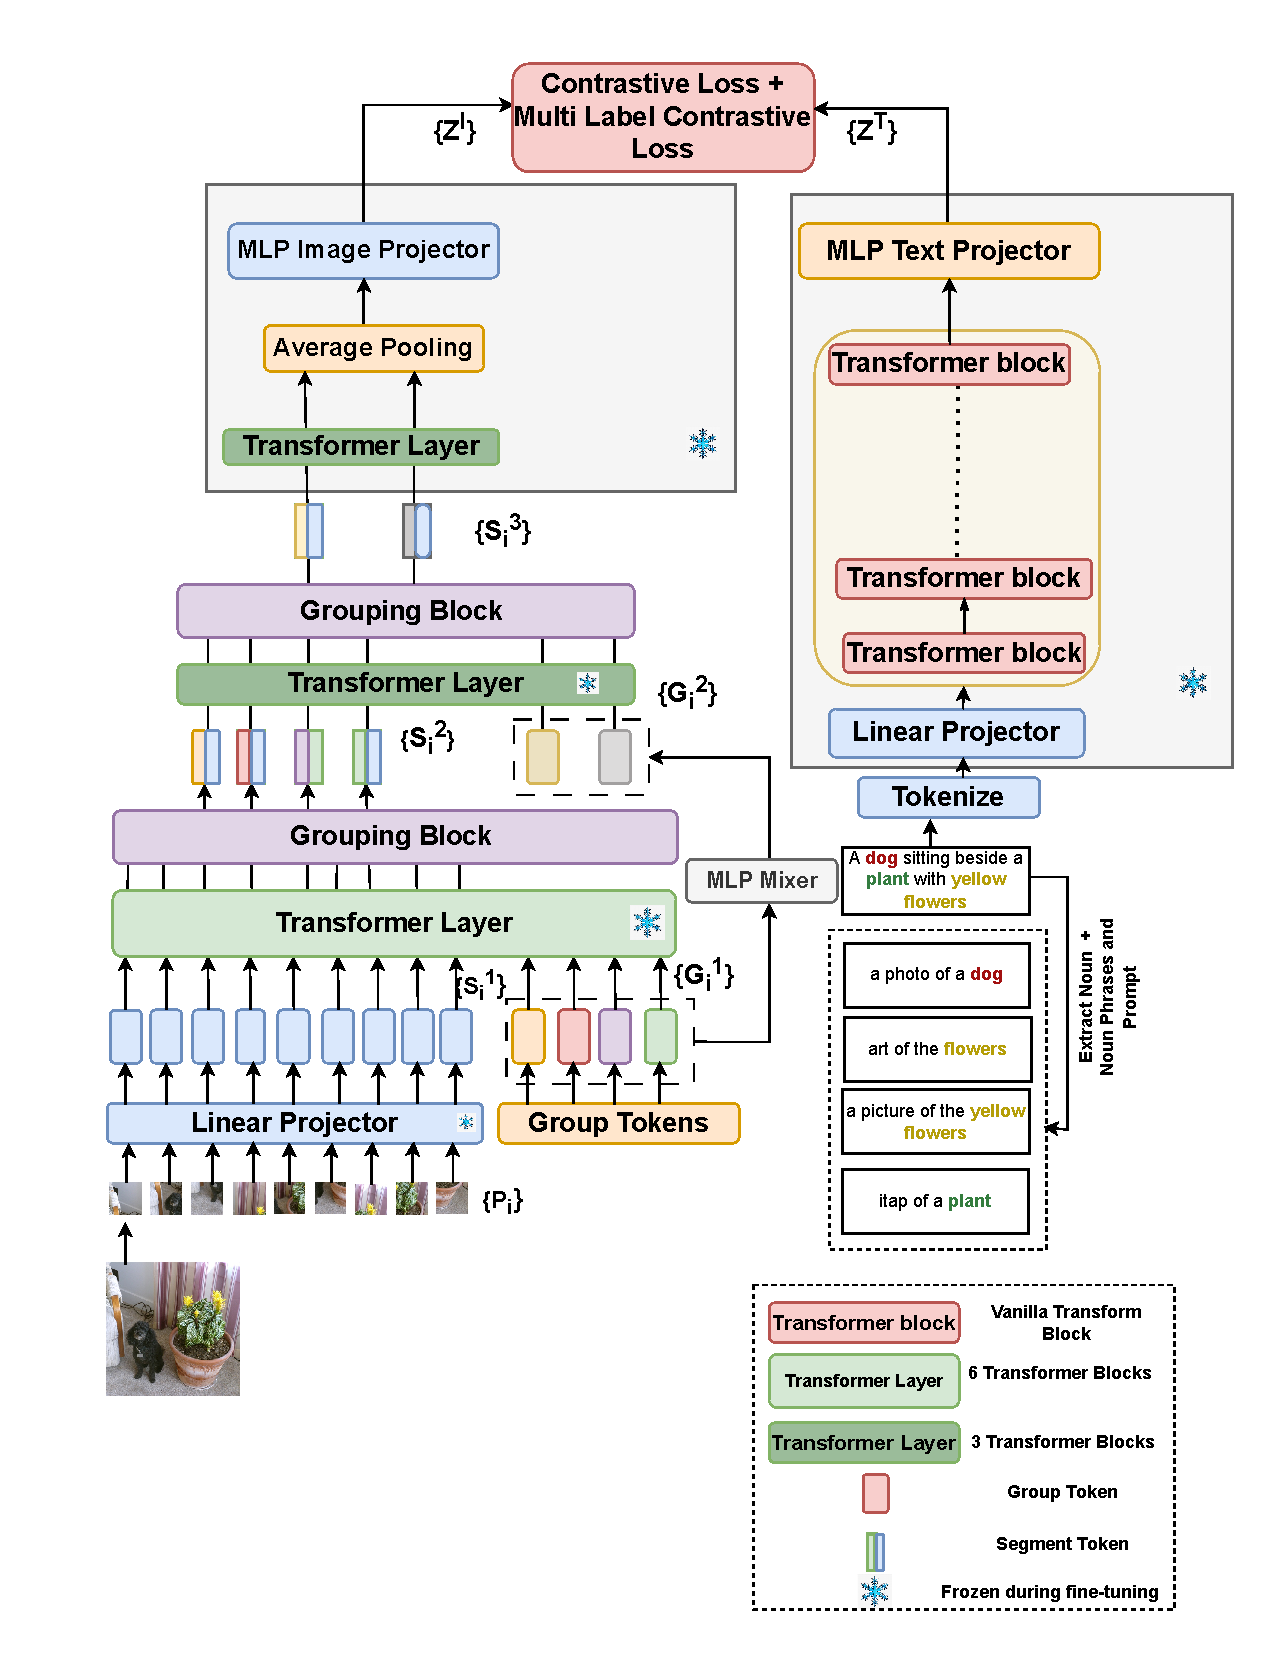
\includegraphics[width=0.91\textwidth]{Images/gvitarch.drawio (5).pdf}
  % \caption{Architecture of GroupViT and Text encoder with contrastive loss}
  \caption[\textbf{GroupViT: Architecture and Training Pipeline}]{\textbf{GroupViT: Architecture and Training Pipeline}. GroupViT employs a hierarchical structure for grouping. Initial stages introduce learnable group tokens to group coherent image concepts via the Grouping Block. Text Encoder processes caption and nouns extracted from caption. Finally, training employs image-text contrastive and multi-label contrastive loss. }
  \label{fig:gvitarch}
\end{figure*}

\begin{figure*}[t!]
  \centering
  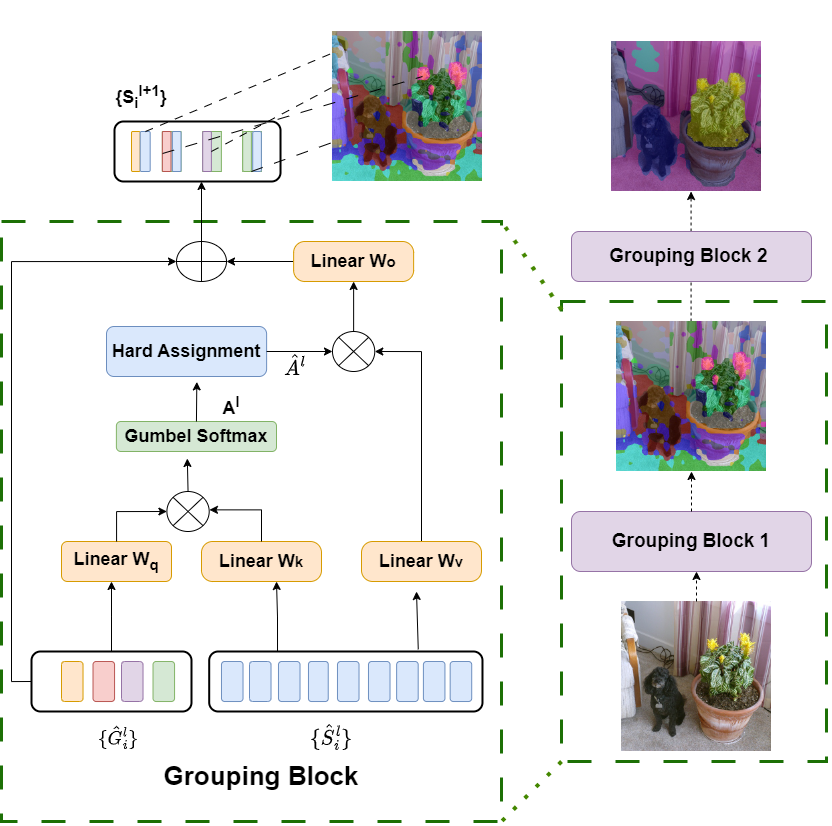
\includegraphics[width=1\textwidth]{Images/GB.drawio (2).drawio (3).png}
  \caption[\textbf{GroupViT: The Architecture of Grouping Block}]{\textbf{GroupViT: The Architecture of Grouping Block}. Each grouping stage
ends with a grouping block that computes the similarity between the learned group tokens and segment (image) tokens. The assignment is
computed via Gumbel-Softmax over group tokens and converted into a one-hot hard assignment. The segment tokens assigned to the same
group are merged together and represent new segment tokens that are input to the next grouping stage.
 }
  \label{fig:groupingblock}
\end{figure*}

\label{sec:gvitarch}
% GroupViT uses transformer-based visual and text encoders to train image-text pairs for semantic segmentation (Figure \ref{fig:gvitarch}). Further details will be discussed in the following sections.

\section{Comparison of similarity/distance measures in discriminating object class}
\label{sec:comparison_same_vs_diff_class}
GroupViT employs multi-stage hierarchy in the vanilla ViT architecture to perform grouping of semantically coherent concepts. Each stage is composed of a Transformer Layer and a Grouping Block. The Transformer layer integrates multiple vanilla Transformer blocks \cite{vaswani2017attention}\cite{dosovitskiy2020image} to execute self-attention that aggregate information globally from all image tokens. Furthermore, a Grouping Block conclude

\begin{figure*}[h]
	\centering
	\begin{subfigure}[b]{0.47\textwidth}
		\centering
		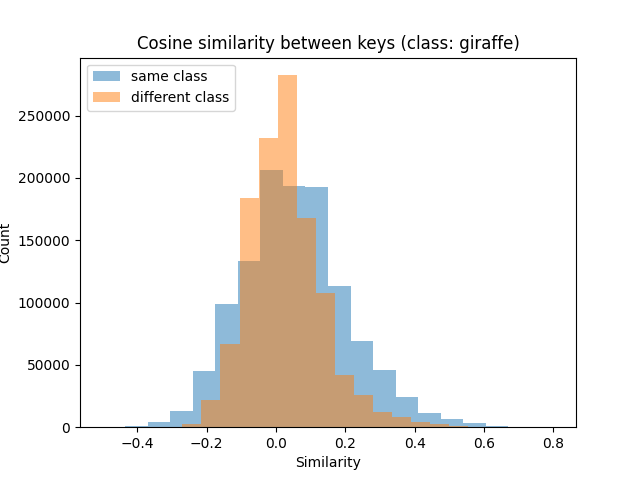
\includegraphics[width=\textwidth]{Images/same_vs_diff_class/plot_giraffe_cosine.png}
		\caption{Cosine similarity}
	\end{subfigure}
	\quad
	\begin{subfigure}[b]{0.47\textwidth}  
		\centering 
		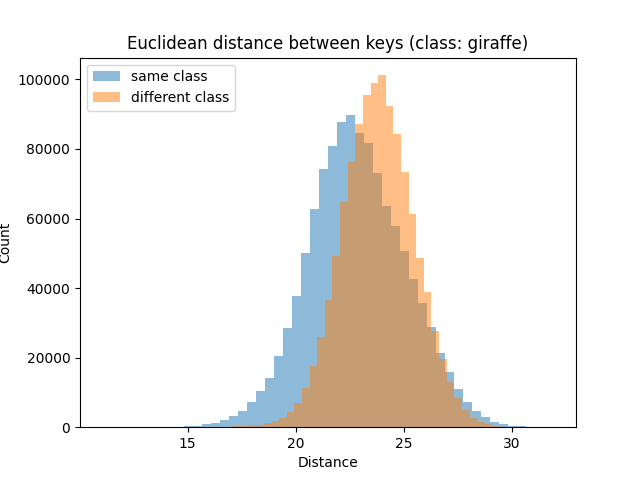
\includegraphics[width=\textwidth]{Images/same_vs_diff_class/plot_giraffe_euc.png}
		\caption{Euclidean}
	\end{subfigure}
	\caption[\textbf{Comparison of keys of images of same and different classes}]{\textbf{Comparison of keys of images of same and different classes}. Shows the pattern of similarity scores and distance measure when comparing keys of same and different classes. Y axis shows number of images compared }
	\label{fig:same_vs_diff}
\end{figure*}

\section{Relaxed best buddies}
\label{sec:comparison_same_vs_diff_class}
GroupViT employs multi-stage hierarchy in the vanilla ViT architecture to perform grouping of semantically coherent concepts. Each stage is composed of a Transformer Layer and a Grouping Block. The Transformer layer integrates multiple vanilla Transformer blocks \cite{vaswani2017attention}\cite{dosovitskiy2020image} to execute self-attention that aggregate information globally from all image tokens. Furthermore, a Grouping Block conclude´

\section{Input data}
During GroupViT training, we utilize image-text pairs as the training data.. 
\subsubsection{Image} 
\label{sec:inputdata}
For images, we integrate various augmentation techniques for model robustness and generalization during training. The augmentation process encompasses color jitter, resizing, cropping, and diverse augment transforms to ensure variability and invariance. We also introduce occluded regions through random erasing to enhance occlusion handling. 
The images are resized to $224 \times 224$ pixels, followed by partitioning into non-overlapping $16 \times 16$ patches with a stride of $16 \times 16$, similar to the Vision Transformer (ViT) methodology \cite{dosovitskiy2020image}. For each image, we split the image into $L = (H \times W)/P^2$ non-overlapping patches with patch size P.
\subsubsection{Text} 
\label{sec:text_aug}
For text, GroupViT extracts nouns from image caption using NLTK \cite{loper2002nltk} and prompts them with a  predefined set of templates having 7 prompts, introduced by Radford et al. in CLIP \cite{radford2021learning}. If NLTK does not extract the required number of labels due to either limited richness in the caption or diversity in the image, GroupViT addresses this by utilizing the associated caption to fulfill the required label count. This ensures a consistent input count for the model.
% Unlike CLIP, which operates at a coarser level, GroupViT aligns image embeddings with extracted nouns through a multi-label loss, improving fine-grained textual-visual alignment.


\section{Vision Encoder}
\label{sec:vision}
% GroupViT employs multi-stage hierarchy in the vanilla ViT architecture to perform grouping of semantically coherent concepts. Each stage is composed of a Transformer Layer and a Grouping Block. The Transformer layer integrates multiple vanilla Transformer blocks \cite{vaswani2017attention}\cite{dosovitskiy2020image} to execute self-attention that aggregate information globally from all image tokens. Furthermore, a Grouping Block concludes each stage, merging smaller groups into larger ones. 
%  Moreover, as illustrated in Fig. \ref{fig:gvitarch}, Unlike ViT, GroupViT avoids passing all image patches through every network layer. Instead, GroupViT undertakes patch grouping in two stages, forwarding the resulting segmented patches to subsequent network layers.
 
% Further elaboration on visual grouping intricacies will be provided in the subsequent sections.\\
% % The backbone ViT-S/16, introduced by Dosovitskiy et al. (2020) is divided into three distinct stages. Each responsible to identify coherent concepts and eventually group them together. First stage is responsible to identify coherence and group them. These grouped segments then form an input for the second stage which grpups these concept into fewer but larger concepts. 
GroupViT utilizes the ViT backbone, enhanced by additional components designed to facilitate the grouping of semantically coherent concepts at different stages within its architecture. The GroupViT model is structured into three stages, with the first two stages culminating in the incorporation of a Grouping Block dedicated to visual grouping.

In GroupViT's earlier stages, there is a Transformer Layer and a Grouping Block. The Transformer layer integrates multiple vanilla Transformer blocks \cite{vaswani2017attention}\cite{dosovitskiy2020image} to aggregate global information from all image tokens. For the first and second stages, a Grouping Block follows the Transformer layer, identifying and merging coherent concepts. Unlike ViT, as shown in Figure \ref{fig:gvitarch}, GroupViT does not process all image patches through each network layer. Instead, it conducts patch grouping and forwards segmented patches to subsequent layers. Further information about visual grouping is presented in upcoming sections.\\
%  the visual encoder accomplishes hierarchical multi-stage grouping.

\textbf{Input Embedding:} 
Image patches are subjected to a linear projection process, projecting them to a higher-dimensional space of 384 dimensions, denoted by $\textbf{P} \in \mathbb{R}^{H \times W \times D}$. Here, $H$ and $W$ correspond to 16, and $D$ is 384. We denote this patch set as $\{\textbf{P}_i\}_{i=1}^{N}$, where $N$ is the number of patch tokens. For positional awareness, positional encoding is integrated into the patch embeddings, utilizing a non-sinusoidal and simple positional encoding scheme. The linear projection employs a single-layer MLP projector with an inner dimension of 384, as shown in Eq. \ref{eq:linearproj}.

\begin{equation}
\label{eq:linearproj}
\{\textbf{S}_i^{1}\}_{i=1}^{N} = \text{Linear\_Projection}(\{\textbf{P}_i\}_{i=1}^{N})
\end{equation}

% As previously indicated, the Visual Encoder comprises three stages. 
The input to each stage is denoted as $\{\textbf{S}_i^{l}\}_{i=1}^{M_0}$, where $M_0$ signifies the segmented tokens grouped by the preceding stage. For the initial stage ($l=1$), $M_0$ is equal to  $N$,  as denoted in Eq. \ref{eq:linearproj}. We introduce learnable parameters for visual grouping in first and second stage, called as group tokens. These group tokens are represented as $\{\textbf{G}_i^{l}\}_{i=1}^{N_0}$, where $N_0$ denotes the number of group tokens. These group tokens are then linearly projected, as the patch tokens, to generate embeddings $\{\textbf{G}_i^{l}\} \in \mathbb{R}^{N_0\times D}$, as shown in Eq. \ref{eq:grouplinearproj}
\begin{equation}
\label{eq:grouplinearproj}
\{\textbf{G}_i^{1}\}_{i=1}^{N_0} = \text{Linear\_Projection}(\{\textbf{G}_i\}_{i=1}^{N_0})
\end{equation}
% For the first stage, $N_0$ is set to 64 and 8 for the second stage.
% We concatenate patch embeddings $\{S_i^{l}\}_{i=1}^{M_0}$ and group embeddings $\{G_i^{l}\}_{i=1}^{N_0}$ to for an input for the transformer layer of GroupViT.

\subsection{Transformer Layer}
% The patch embeddings are combined with 64 learnable group token embeddings introduced for visual grouping, resulting in the input to these transformer blocks. 
The Transformer layer compromises of multiple Vanilla Transformer block, introduced by Vaswani et al. \cite{vaswani2017attention}. For stages with group tokens in the visual encoder, we concatenate the segment embeddings $\{\textbf{S}_i^{l}\}_{i=1}^{M_0}$ and the group token embeddings $\{\textbf{G}_i^{l}\}_{i=1}^{N_0}$, as denoted by the `;' operator in Eq. \ref{eq:transformer}.
This concatenated input is propagated through self-attention blocks facilitating information propagation. We denote the output from the transformer layer as  $\{\hat{\textbf{S}_i^{l}}\}$ and $\{\hat{\textbf{G}_i^{l}}\}$ for segment tokens and group token respectively as in Eq. \ref{eq:transformer}
\begin{equation}
\label{eq:transformer}
    \{\hat{\textbf{G}_i^{l}}\}, \{\hat{\textbf{S}_i^{l}}\} = \text{Transformer}(\{\textbf{G}_i^{l}\}; \{\textbf{S}_i^{l}\})
\end{equation}

\subsection{Grouping Block}
Grouping Block merges all the segment tokens that are assigned to the same group token into a single new image segment, which we call Segment Token. This grouping is based on similarity.
For better comprehension, we break down the grouping mechanism into two main steps:(i) computing attention to assess the similarity between individual patch tokens and group tokens, and (ii) assigning each patch token to one of the group tokens based on the derived similarity scores.
\subsubsection{Attention}
Before Grouping Block, the model de-concatenates the segment token embeddings and group token embeddings. The Grouping Block, depicted in Fig. \ref{fig:groupingblock}, takes $\{\hat{\textbf{G}_i^{l}}\}$ and $\{\hat{\textbf{S}_i^{l}}\}$ as inputs to perform cross-attention. For cross-attention, $\{\hat{\textbf{G}_i^{l}}\}$ serves as $q$ and $\{\hat{\textbf{S}_i^{l}}\}$ serves as $k$ and $v$. The $q$, $k$, and $v$ are subsequently linearly projected using weights $\textbf{W}_q$, $\textbf{W}_k$, and $\textbf{W}_v$ to obtain query, key, and value. Then, we compute the similarity matrix $\textbf{A}^{l}$ by Gumbel-Softmax \cite{jang2016categorical}\cite{maddison2016concrete}, as shown in Eq. \ref{eq:gumbel}. Here, $\gamma$ is randomly drawn from the gumbel distribution.
The obtained value $\textbf{A}^{l}$ is referred as \textbf{soft attention}.

\begin{equation}
\begin{aligned}
\label{eq:gumbel}
\textbf{A}^{l}_{i,j} = \frac{\exp(\textbf{W}_q\hat{\textbf{G}}_i^{l} \cdot \textbf{W}_k\hat{\textbf{S}}_j^{l} + \gamma_i)}{\sum_{k=1}^{M_l} \exp(\textbf{W}_q\hat{\textbf{G}}_i^{l} \cdot \textbf{W}_k\hat{\textbf{S}}_j^{l} + \gamma_k)}
\end{aligned}
\qquad
\text{, where $\gamma \in (0, 1)$.}
\end{equation}

\subsubsection{Assignment}
We determine the segment token's assigned group by finding the group with the highest value through the one-hot operation over the soft attention calculated above in Eq. \ref{eq:gumbel}. We use the straight-through trick \cite{van2017neural} to enable differentiation of the non-differentiable one-hot assignment operation, ensuring smooth gradient flow for training purposes, as demonstrated in Equation \ref{eq:hardassignment}. Here, $\text{sg}$ represents the stop gradient operator. 
\begin{equation}
\label{eq:hardassignment}
\hat{\textbf{A}}^l = \text{OneHotAssignment}(\text{argmax}(\textbf{A}^l)) + \textbf{A}^l - \text{sg}(\textbf{A}^l),
\end{equation}
The obtained value of $\hat{\textbf{A}}_l$ is referred as \textbf{hard assignment} and reflects the assignment of segment tokens to a single group token.
 % $\hat{\textbf{A}}_l$ to assume a one-hot value,reflecting the assignment of a single group, 
 % while maintaining a gradient aligned with $A_l$. This property guarantees the differentiability and end-to-end trainability of the Grouping Block. This method of assignment is known as "hard assignment."

Once the segment tokens are assigned to various learned groups using the hard assignment, the embeddings of tokens within the same group are aggregated to create a new segment token $\mathbf{S}^{l+1}_{i}$. For each group, we obtain the weighted sum of segment tokens assigned to that group and finally project the merged features using a learnable linear weight matrix $\mathbf{W}_o$, as shown in Equation \ref{eq:grouping_output}. Together with $\mathbf{G}_i^{l}$, we form the output segment tokens for the next stage, denoted as $\mathbf{S}^{l+1}_{i}$, as shown in Equation \ref{eq:grouping_output}.

\begin{equation}
\label{eq:grouping_output}
{\textbf{S}}^{l+1}_{i} = \textbf{G}_i^{l} + \frac{\sum_{j=1}^{M_{l-1}} \hat{\textbf{A}}_l(i,j){\textbf{W}}_{v}\hat{\textbf{S}}^l_j}{\sum_{j=1}^{M_{l-1}} \hat{\textbf{A}}_l(i,j)}
\end{equation}

% \begin{equation}
% \label{eq:groupedfinal}
%  {\textbf{S}}^{l+1}_{i} = \textbf{G}_i^{l} + \ddot{\textbf{S}}^{l+1}_{i}
% \end{equation}

We visualize the concepts learned by a few Group Tokens from stage 2 in Fig \ref{fig:conceptslearnedbygt}, where we observe Group 0 learns semantics of `horse' and Group 5 learns semantics of `person'. It is important to note that one group can learn multiple concepts as visualized in Fig. \ref{fig:multiconceptslearnedbygt} where we observe Group 0 learns multiple concepts in different images such as `aeroplane', `bird', `horse' and `sheep'

% \begin{equation}
% \label{eq:grouping_output}
% \hat{S}^{l+1}_{i} = G_i^{l} + W_o {\sum_{j=1}^{M_l-1} \hat{A}^{l}_{i,j} W_v \hat{S}_l^{j}} 

% % {\sum_{j=1}^{M_l-1} \hat{A}_{l,i,j}}
% \end{equation}



% \begin{equation}
% \label{eq:hardassignment}
%     \{\hat{S_i^{l+1}}\} = \text{GumbelSoftmax}\left(\frac{query(key)^T}{\sqrt{D}}\right)
% \end{equation}
\subsection{Multi-stage Information Flow}
After detailing the components of each stage, we now present the end-to-end flow of information within the visual encoder. GroupViT follows a three-stage approach: the initial stage consists of 6 transformer blocks and 64 learnable group tokens, represented as $\{\textbf{G}_i^{1}\}$ in Fig. \ref{fig:gvitarch}, with $\{\textbf{S}_i^{1}\}$ segment tokens. The Grouping Block merges all the segment tokens that are assigned to the same group token into a single new image segment, resulting in 64 segments, denoted as $\{\textbf{S}_i^{2}\}$ in Fig. \ref{fig:gvitarch}. The second stage comprises 3 transformer blocks, which take $\{\textbf{S}_i^{2}\}$ and 8 group tokens, depicted as $\{\textbf{G}_i^{2}\}$ in Fig. \ref{fig:gvitarch}. The Grouping Block further merges coherent concepts into new segment tokens, generating 8 segments, labeled as $\{\textbf{S}_i^{3}\}$ in Fig. \ref{fig:gvitarch}. In the final stage, 3 transformer blocks process $\{\textbf{S}_i^{3}\}$ as input, without any group tokens. This gradual reduction in the number of group tokens aims to create larger and fewer segment tokens through similarity-based grouping. This progression is symbolized by the successive narrowing of the width of Grouping Blocks and Transformer layers from stage 1 to stage 3 in Fig. \ref{fig:gvitarch}.

On second stage, we also integrate the information of learned group tokens of first stage into fresh learnable tokens of stage 2. To handle the difference in group token numbers in the second and first stage, an MLP-Mixer is applied \cite{tolstikhin2021mlp}, as shown in Eq. \ref{eq:mlpmixer}, and visualized in Fig. \ref{fig:gvitarch}\\
\begin{equation}
\label{eq:mlpmixer}
    \{\textbf{G}_i^{2}\} =  \{\textbf{G}_i^{2}\} + \text{MLPMixer}(\{\textbf{G}_i^{1}\})
\end{equation}
In the third stage, we do not introduce new group tokens, so we pass the output of the second stage directly to the final stage. Unlike the previous stages, the third stage lacks a grouping block and concludes with the application of Average Pooling on segment embeddings, as shown in Fig. \ref{fig:gvitarch}. This process results in a condensed image representation which we project  into a multi-modal feature embedding space, as visualized in Fig. \ref{fig:gvitarch}. By doing so, we  obtain $\textbf{Z}^I \in \mathbb{R}^{1 \times D_J}$, where $D_J$ signifies the dimensionality of the joint latent space corresponding to a 256-dimensional space, shown in Eq. \ref{eq:imgproj}. To accomplish this, a 2-layer MLP projector is employed, having an inner dimension of 4096 and an output dimension of 256.

\begin{equation}
\label{eq:imgproj}
    \{\textbf{Z}^I \} = \text{MLP}(\text{Average\_Pool}( \{{\hat{\textbf{S}}_i^{3}}\}))
\end{equation}

% \begin{equation}
% \label{eq:imgproj}
% \{\textbf{Z}^I \} = \text{MLP}(\{\hat{\textbf{S}_i^{3}}\})
% \end{equation}

In conclusion, the multi-stage visual encoder conducts visual grouping, leading to the gradual emergence of fewer and larger coherent concepts. This process culminates in the projection of a singular image embedding obtained through average pooling into the shared joint embedding space.


\subsection{Text Encoder}
\label{sec:textencoder}

% The text-encoder consists of 12 self-attention transformer blocks, as introduced by Vaswani et al. \cite{vaswani2017attention}, operating with a 256-dimensional embedding. Extracted labels and captions, as outlined in Section \ref{sec:text_aug}, are tokenized and subjected to embedding generation. These embeddings then traverse the text encoder following Eq. \ref{eq:txtencode}, generating embeddings for each label, denotes as $\hat{T_i^{L+1}} \in \mathbb{R}^{\{L+1\} \times D_T}$, where $D_T$ represents the dimensional space of text encoder, set to 256 for GroupViT . Following this, the embeddings are passed through an MLP projector to project them into a multi-modal feature space, generating $Z_T^{L+1} \in \mathbb{R}^{\{L+1\} \times D_J}$, where $D_J$ represents the dimensional space of text encoder
The Text Encoder is composed of 12 self-attention Transformer blocks, following the architecture introduced by Vaswani et al. \cite{vaswani2017attention}. It employs a dimensional space of 256. The extracted labels and captions, detailed in Section \ref{sec:text_aug}, undergo tokenization and are subsequently projected into a text dimension space, denoted as $D_T$, by using a linear projector. We further add positional encodings for sequential information in the generated input embeddings and forward it to the text encoder. This results in embeddings for each label.

Following this, the embeddings proceed through an MLP projector, leading to their projection into a multi-modal feature space. This projection yields $\mathbf{Z}^T_{K+1} \in \mathbb{R}^{\{K+1\} \times D_J}$. Here, $K+1$ denotes `K' extracted labels and the caption, and $D_J$ denotes the dimensionality of the joint embedding space.

\begin{equation}
\label{eq:textproj}
 {\textbf{Z}^T_{K+1}} = \text{MLP}(\text{TextEncoder}( {\textbf{T}_{K+1}}))
\end{equation}

% \begin{equation}
% \label{eq:textproj}
% {\textbf{Z}^T_{K+1}} = \text{MLP}( {\hat{\textbf{T}}}_{K+1})
% \end{equation}

During the training process, the caption embedding serves for contrastive loss, while the embeddings corresponding to the extracted nouns are utilized for multi-label contrastive loss. We consider the end-of-sentence token embedding from the text encoder as the overall representation of the text. We will explain these losses in detail in the next section \ref{sec:loss}.


\newcommand{\group}[7]{
\begin{subfigure}{\linewidth}\begin{adjustbox}{width=\textwidth}{\def\arraystretch{0.2}\setlength\tabcolsep{#1pt}\begin{tabular}{ccccc}
\raisebox{1.2\normalbaselineskip}[0pt][0pt]{\rotatebox{90}{\tiny #2}} &
\includegraphics[height=2cm]{figures/#7/#3} &
\includegraphics[height=2cm]{figures/#7/#4} &
\includegraphics[height=2cm]{figures/#7/#5} &
\includegraphics[height=2cm]{figures/#7/#6} \\
\end{tabular}}\end{adjustbox}\end{subfigure}}

\begin{figure}[thp]
\centering
\vspace{-0.5em}
\group{0.5}{\textbf{Image}}{0050.jpg}{0008.jpg}{0023.jpg}{0024.jpg}{group0}

\group{0.5}{\textbf{Group 0}}{0050attn_map0withouttitle.png}{0008attn_map0withouttitle.png}{0023attn_map0withouttitle.png}{0024attn_map0withouttitle.png}{group0}
\group{0.5}{\tiny \textbf{Image}}{0004.jpg}
{0007.jpg}
{0031.jpg}
{0009.jpg}
{group5}
\group{0.5}{\tiny \textbf{Group 5}}
{0004attn_map5withouttitle.png}
{0007attn_map5withouttitle.pdf}
{0031attn_map5withouttitle.png}
{0009attn_map5withouttitle.pdf}
{group5}

\caption[\textbf{Visualization of concepts learned by Group Tokens}]{\textbf{Visualization of concepts learned by Group Tokens in the final stage}. We visualize 
 the concepts learned by Group 0 in top row and Group 5 in bottom row. Group 0 learns `horse', while Group 5 learns `person'.}
\label{fig:conceptslearnedbygt}
\end{figure}



\begin{figure}[thp]
\centering
  \vspace{-0.5em}

\group{0.5}{\textbf{\footnotesize Image}}{0000.jpg}{0074.jpg}{0023.jpg}{0030.jpg}{group0}
\group{0.5}{\textbf{\footnotesize Group 0}}{0000attn_map0withouttitle.png}{0074attn_map0withouttitle.png}{0023attn_map0withouttitle.png}{0030attn_map0withouttitle.png}{group0}

\caption[\textbf{Visualization of multiple concepts learned by a Group Token}]{\textbf{Visualization of multiple concepts learned by Group Token 0 in the final stage}. We visualize 
 the multiple concepts such as `aeroplane', `bird', `horse' and `sheep', learned by Group 0, demonstrating that a single group token can capture multiple semantic concepts. }
\label{fig:multiconceptslearnedbygt}
\end{figure}

\section{Training Loss}

\subsection{Contrastive loss}
\label{sec:loss}
 We employ a noisy image-text pair contrastive loss, as previously utilized by Radford et al. for the CLIP model \cite{radford2021learning} and by Jia et al. for the ALIGN model \cite{jia2021scaling}. In the training process, we consider a batch of size $B$ containing image-text pairs $\{(x^{I}_i, x^T_i)\}_{i=1}^B$, where $x^I_i$ and $x^T_i$ represent the image and text inputs of the $i$-th pair, respectively. These inputs are encoded using their respective encoders to obtain embedding vectors $Z^I_i$ and $Z^T_i$, which are then l2-normalized. The paired image-text data is treated as positive examples, while other pairs serve as negatives. 
\textbf{The image-to-text contrastive loss:}
\begin{equation}
L_{I\rightarrow T} = -\frac{1}{B} \sum_{i=1}^{B} \log \frac{\exp(\textbf{Z}^I_i \cdot \textbf{Z}^T_i / \tau)}{\sum_{j=1}^{B} \exp(\textbf{Z}^I_i \cdot \textbf{Z}^T_j / \tau)}
\end{equation}

\textbf{The text-to-image contrastive loss:}
\begin{equation}
L_{T\rightarrow I} = -\frac{1}{B} \sum_{i=1}^{B} \log \frac{\exp(\textbf{Z}^T_i \cdot \textbf{Z}^I_i / \tau)}{\sum_{j=1}^{B} \exp(\textbf{Z}^T_i \cdot \textbf{Z}^I_j / \tau)}
\end{equation}

\textbf{The bidirectional loss:}
\begin{equation}
\label{eq:cl}
L_{I \leftrightarrow \{T_k\}_{k=1}^K} = L_{I\rightarrow \{T_k\}_{k=1}^K} + L_{\{T_k\}_{k=1}^K \rightarrow I}
\end{equation}

These equations capture the loss functions used in GroupViT for aligning image and text representations during training.


\subsection{Multi-label Contrastive Loss}
\label{sec:mll}

In tandem with the Contrastive loss, GroupViT introduces a multi-label contrastive loss to enrich the discriminatory potential of the acquired representation space. This enhancement is particularly relevant for tasks requiring a level of granularity beyond that covered by models like CLIP and ALIGN. To achieve this, GroupViT leverages extracted labels from captions, as discussed in Section \ref{sec:text_aug}. All the corresponding `K' prompted labels are employed as positives, while the remaining $B(K-1)$ are treated as negatives within the multi-label contrastive loss framework. While it is plausible that embeddings of identical nouns could be treated as negatives in this scenario, it's essential to emphasize that the ALIGN model underscores the ability of large web-scaled dataset to offset the presence of noisy image-text pairs. The formulation of this loss is presented in Equation \ref{eq:mll}.\\
\textbf{The image-to-text multi-label contrastive loss:}
\begin{equation}
\label{eq:mll}
\mathcal{L}_{I \rightarrow \{T_k\}_{k=1}^K} = -\frac{1}{B}\sum_{i=1}^{B} \log \left( \frac{\sum_{k=1}^{K} \exp(\textbf{Z}^I_i \cdot \textbf{Z}^{T_k}_i/\tau)}{\sum_{k=1}^{K} \sum_{j=1}^{B} \exp(\textbf{Z}^I_i \cdot \textbf{Z}^{T_k}_j/\tau)} \right)
\end{equation}
\textbf{The text-to-image multi-label contrastive loss:}\\
\begin{equation}
\mathcal{L}_{\{T_k\}_{k=1}^K \rightarrow I} = -\frac{1}{KB}\sum_{k=1}^{K} \sum_{i=1}^{B} \log \frac{\exp(\textbf{Z}^{T_k}_i \cdot \textbf{Z}^{I}_i/\tau)}{\sum_{j=1}^{B} \exp(\textbf{Z}^{T_k}_i \cdot \textbf{Z}^{I}_j/\tau)}
\end{equation}
\textbf{The bidirectional loss:}
\begin{equation}
\mathcal{L}_{I \leftrightarrow \{T_k\}_{k=1}^K} = \mathcal{L}_{I \rightarrow \{T_k\}_{k=1}^K} + \mathcal{L}_{\{T_k\}_{k=1}^K \rightarrow I}
\end{equation}


%\begin{figure}[htbp]
\label{fig:groupsonstages}
  \centering
  
  \vspace{-0.5em}
  \subfloat[Image]{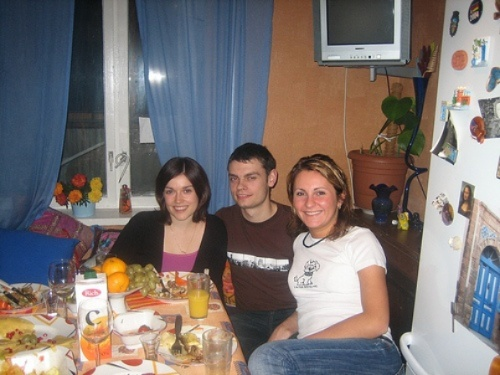
\includegraphics[width=0.24\textwidth]{figures/experiments/results_orckpt/44/0044.jpg}}
  \hfill
  \subfloat[Mask Prediction]{
\includegraphics[width=0.24\textwidth]{figures/experiments/results_orckpt/44/0044.png}}
  \hfill
  \subfloat[Grouping: Stage 1]{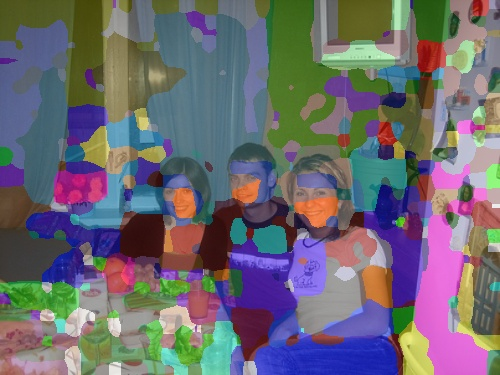
\includegraphics[width=0.24\textwidth]{figures/experiments/results_orckpt/44/0044_layer0.jpg}}
  \hfill
  \subfloat[Grouping: Stage 2]{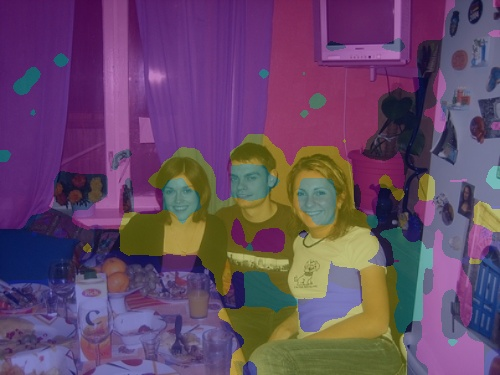
\includegraphics[width=0.24\textwidth]{figures/experiments/results_orckpt/44/0044_layer1.jpg}}
  
  \vspace{-0.5em}
 
  \subfloat[Group 1]{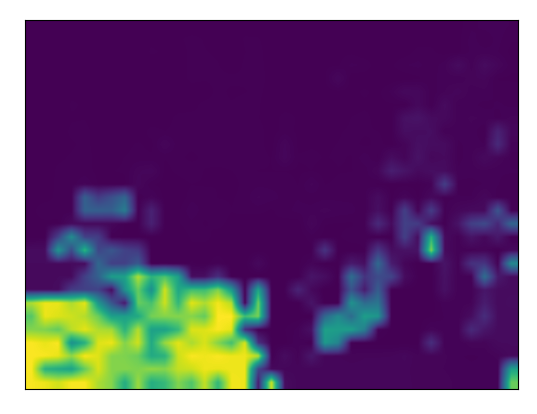
\includegraphics[width=0.24\textwidth]{figures/experiments/results_orckpt/44/attn_map0withouttitle.png}}
  \hfill
  \subfloat[Group 2]{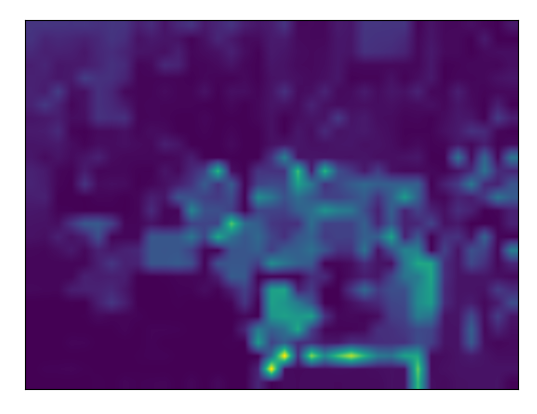
\includegraphics[width=0.24\textwidth]{figures/experiments/results_orckpt/44/attn_map1withouttitle.png}}
  \hfill
  \subfloat[Group 3]{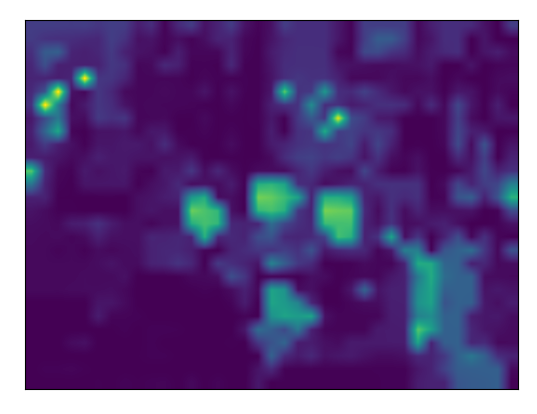
\includegraphics[width=0.24\textwidth]{figures/experiments/results_orckpt/44/attn_map2withouttitle.png}}
  \hfill
  \subfloat[Group 4]{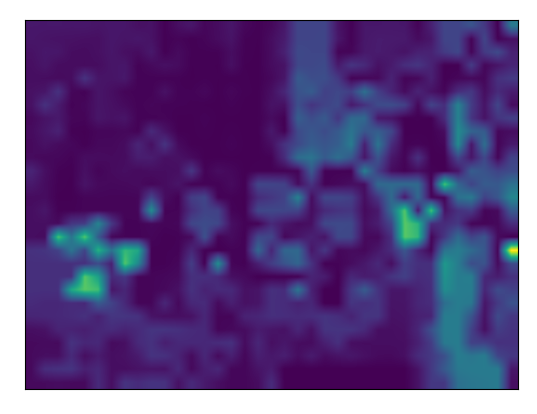
\includegraphics[width=0.24\textwidth]{figures/experiments/results_orckpt/44/attn_map3withouttitle.png}}
  
  \vspace{-0.5em}
 
  \subfloat[Group 5]{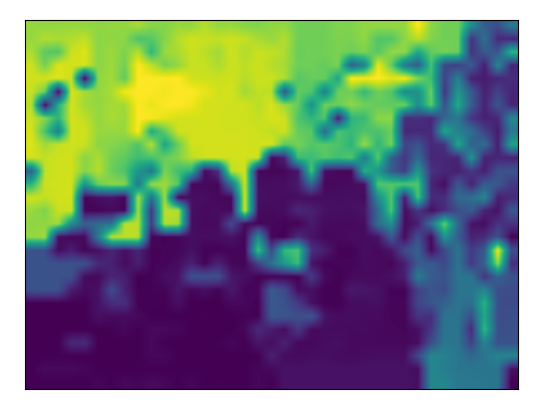
\includegraphics[width=0.24\textwidth]{figures/experiments/results_orckpt/44/attn_map4withouttitle.png}}
  \hfill
  \subfloat[Group 6]{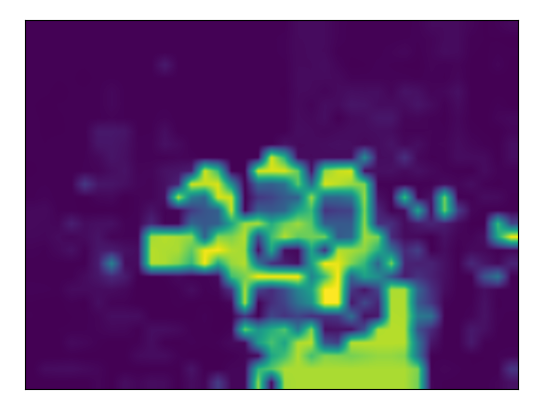
\includegraphics[width=0.24\textwidth]{figures/experiments/results_orckpt/44/attn_map5withouttitle.png}}
  \hfill
  \subfloat[Group 7]{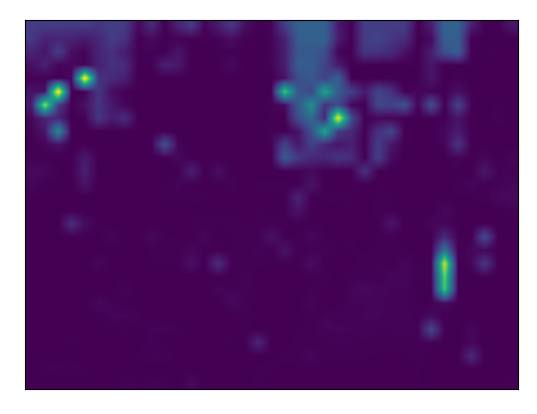
\includegraphics[width=0.24\textwidth]{figures/experiments/results_orckpt/44/attn_map6withouttitle.png}}
  \hfill
  \subfloat[Group 8]{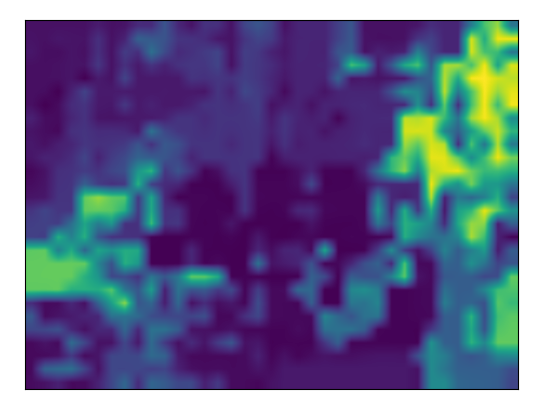
\includegraphics[width=0.24\textwidth]{figures/experiments/results_orckpt/44/attn_map7withouttitle.png}}
   
  \caption{\textbf{Visualization of Grouping Mechanism}}
  \label{fig:group_vis}
\end{figure}

\begin{figure}[htbp]
  \centering

  \vspace{-0.5em}
  \subfloat[Image ii]{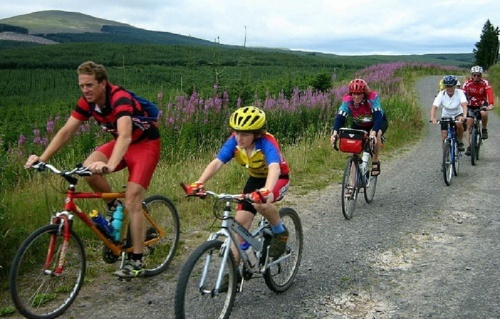
\includegraphics[width=0.24\textwidth]{figures/experiments/results_orckpt/39/0039_image.jpg}}
  \hfill
  \subfloat[Mask Prediction]{
\includegraphics[width=0.24\textwidth]{figures/experiments/results_orckpt/39/0039.png}}
  \hfill
  \subfloat[Grouping: Stage 1]{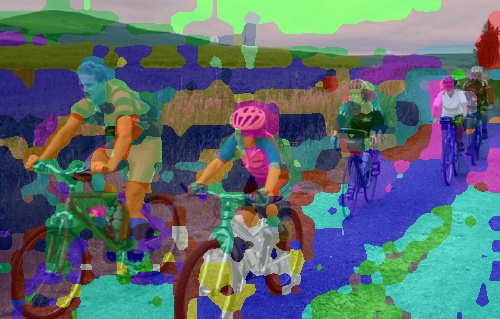
\includegraphics[width=0.24\textwidth]{figures/experiments/results_orckpt/39/0039_layer0.jpg}}
  \hfill
  \subfloat[Grouping: Stage 2]{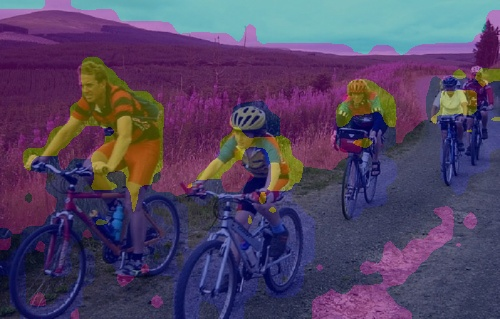
\includegraphics[width=0.24\textwidth]{figures/experiments/results_orckpt/39/0039_layer1.jpg}}
  
  \vspace{-0.5em}
 
  \subfloat[Group 1]{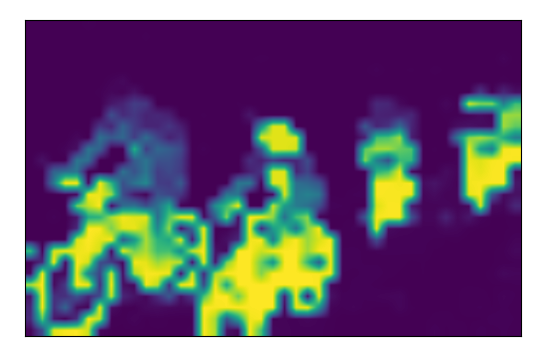
\includegraphics[width=0.24\textwidth]{figures/experiments/results_orckpt/39/attn_map0withouttitle.png}}
  \hfill
  \subfloat[Group 2]{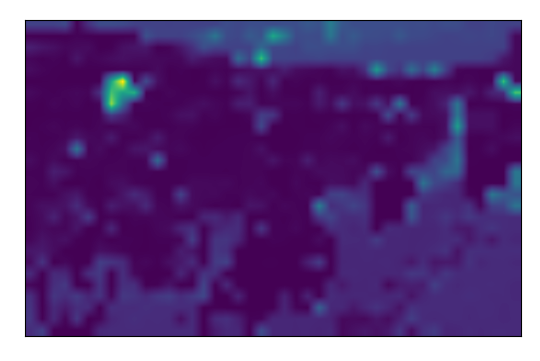
\includegraphics[width=0.24\textwidth]{figures/experiments/results_orckpt/39/attn_map1withouttitle.png}}
  \hfill
  \subfloat[Group 3]{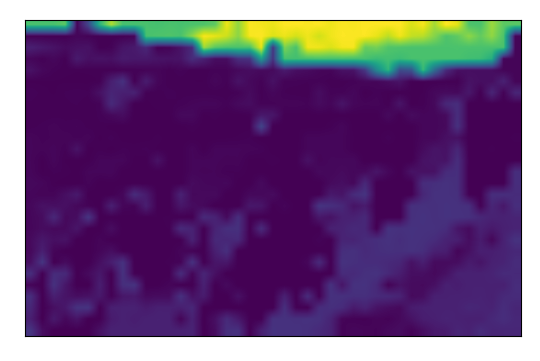
\includegraphics[width=0.24\textwidth]{figures/experiments/results_orckpt/39/attn_map2withouttitle.png}}
  \hfill
  \subfloat[Group 4]{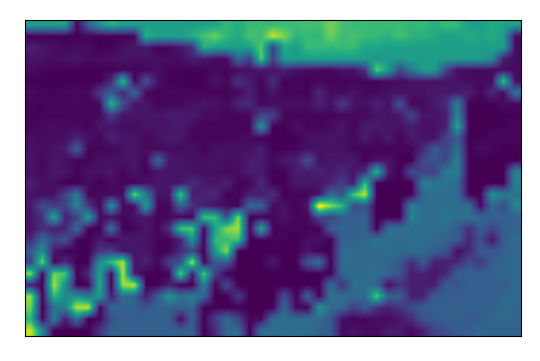
\includegraphics[width=0.24\textwidth]{figures/experiments/results_orckpt/39/attn_map3withouttitle.png}}
  
  \vspace{-0.5em}
 
  \subfloat[Group 5]{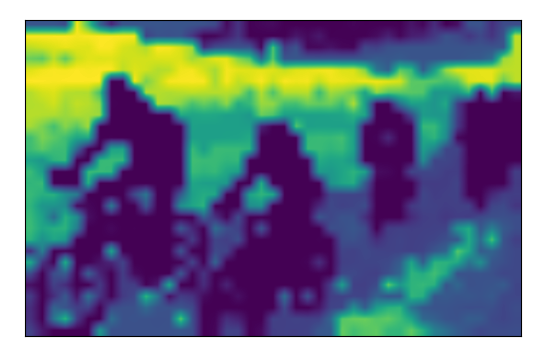
\includegraphics[width=0.24\textwidth]{figures/experiments/results_orckpt/39/attn_map4withouttitle.png}}
  \hfill
  \subfloat[Group 6]{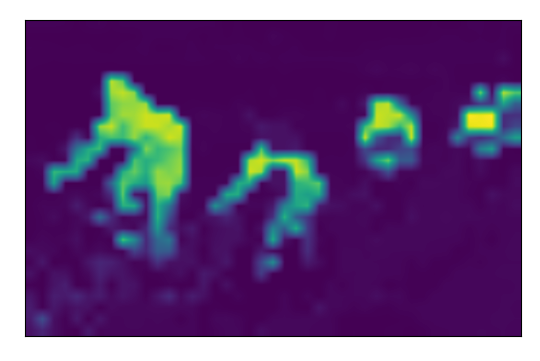
\includegraphics[width=0.24\textwidth]{figures/experiments/results_orckpt/39/attn_map5withouttitle.png}}
  \hfill
  \subfloat[Group 7]{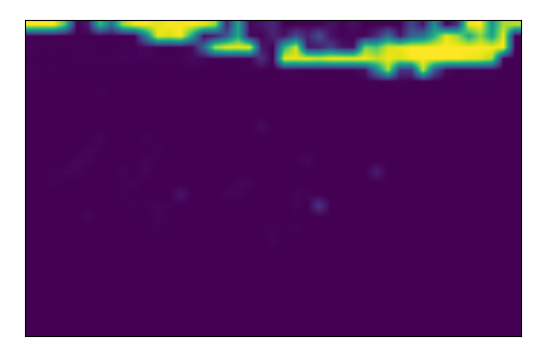
\includegraphics[width=0.24\textwidth]{figures/experiments/results_orckpt/39/attn_map6withouttitle.png}}
  \hfill
  \subfloat[Group 8]{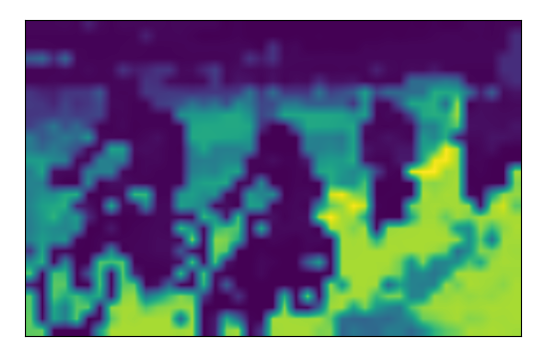
\includegraphics[width=0.24\textwidth]{figures/experiments/results_orckpt/39/attn_map7withouttitle.png}}

  \caption{Visualization of Grouping Mechanism (cont'd)}
  \label{fig:group_vis_contd}
\end{figure}



\section{Inference}
\label{sec:inf}
\begin{figure*}
  \centering
  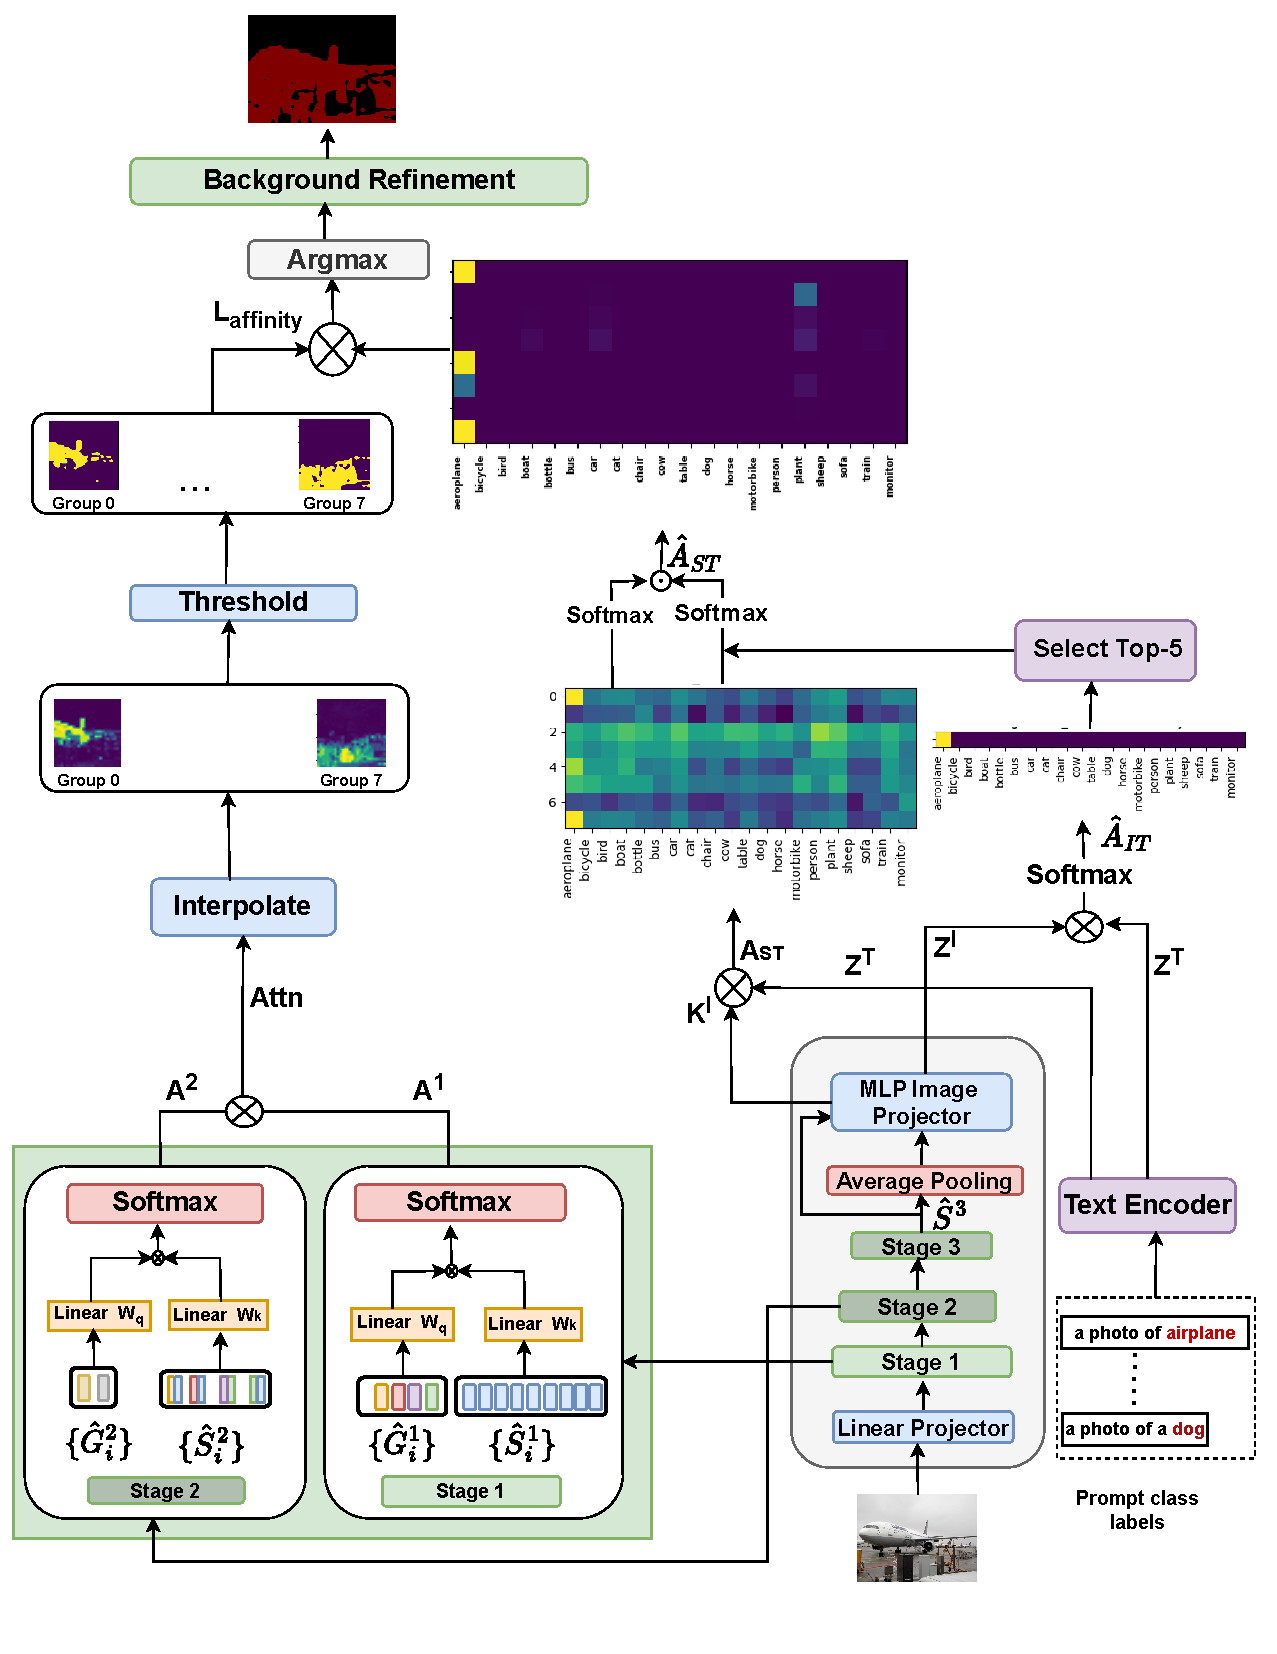
\includegraphics[width=1\textwidth, height=0.8\textheight]{Images/temp.drawio (4).pdf}
  \caption[\textbf{GroupViT: Inference Pipeline}]{\textbf{GroupViT Inference Pipeline. }GroupViT calculates similarity between the average image embedding and text embeddings ($\textbf{A}_{IT}$) and between segment embeddings and class label embeddings ($\textbf{A}_{ST}$). The top-5 classes are selected from $\textbf{A}_{IT}$, and retained in $\textbf{A}_{ST}$. After obtaining global attention, it resizes and thresholds the attention maps. Finally, it labels the image based on $L_{affinity}$.}
\label{fig:inf}
\end{figure*}

%\todo{These experiment details should come last}
% we use an image resolution of 
% 448x448 
% for the COCO-Object dataset and 0.8 as the background threshold. For the PASCAL VOC 2012 dataset, we use an image resolution of 448x448 and a background threshold of 0.95.
The inference process of GroupViT encompasses two primary tasks: (i) identifying visual groups and (ii) assigning labels to these groups. This section provides a comprehensive breakdown of each stage within the inference process.

% = using attention maps to identify relevant group tokens for each class name. This allows us to make predictions based on the similarity between the image and the class descriptions.
\subsection{Class Descriptive Prompts}
For inference, we utilize class labels to generate text embeddings. To create class descriptive prompts, we use a simple template: `A photo of \{classname\}'. Given N categories, we represent the resulting input embeddings as $\textbf{T} \in \mathbb{R}^{N \times D_T}$. These embeddings are forwarded to the text encoder and an MLP projector to obtain $\textbf{Z}^T \in \mathbb{R}^{N \times D_J}$ in the joint feature space, as shown in Eq. \ref{eq:textproj}

\subsection{Image and Text Alignment}

\subsubsection{Affinity Metric between Segments and Classes}
During inference, similar to the training process, we pass image embeddings through the visual encoder following the approach outlined in Section \ref{sec:vision}. First, as in Eq. \ref{eq:imgproj}, we obtain $\textbf{Z}^I \in \mathbb{R}^{1 \times D_{J}}$, where $D_{J}$ represents the dimension of the multi-modal feature space. Along with obtaining the average embedding  $\textbf{Z}^I$, we further project $\hat{\textbf{S}}^3$ into the joint multi-modal feature space, as shown in Eq. \ref{eq:imgprojbeforeavgpool}. The resulting embeddings are denoted as $\textbf{K}^I$, where ${\textbf{K}^I} \in \mathbb{R}^{\hat{S}^3 \times D_J}$, with $\hat{S}^3$ representing the number of segments after the third and final stage.
\begin{equation}
\label{eq:imgprojbeforeavgpool}
    \textbf{K}^I = \text{MLP}( \hat{\textbf{S}}_i^{3})
\end{equation}

 Following this, we proceed to compute the similarity between the segment embeddings and the class label embeddings in the joint feature space. We label this metric as the `\textbf{segment affinity metric}', denoted by $\textbf{A}_{ST} \in \mathbb{R}^{|S^3| \times N}$.
\begin{equation}
\label{eq:simmat}
\text{$\textbf{A}_{ST}$}   =  \textbf{K}^I \cdot \text{Transpose}(\textbf{Z}^T)
\end{equation}

% Moving forward, we subject the similarity metric to a softmax operation, resulting in a probabilistic distribution along the last dimension, as in Eq. \ref{eq:softmaxsimmat}.


% \begin{equation}
% \label{eq:softmaxsimmat}
% \ddot{\textbf{A}}_{ST} = \text{Softmax}(\textbf{A}_{ST})
% \end{equation}


\subsubsection{Average Affinity Metric}
We further compute the similarity between $\textbf{Z}^I$ and the text embeddings $\textbf{Z}^T$ in the joint feature space. This obtained metric is referred to as the `\textbf{average image affinity metric}' and is represented as $A_{IT} \in \mathbb{R}^{1 \times N}$, where N is the number of class labels. This can be seen in Eq. \ref{eq:avgsimilarity}

\begin{equation}
\label{eq:avgsimilarity}
    \text{$\textbf{A}_{IT}$} = \{\textbf{Z}^I\} \cdot \{\textbf{Z}^T\}^T
\end{equation}

To convert the obtained values into a probabilistic distribution, we apply the softmax function along the last dimension.
\begin{equation}
\label{eq:softmaxavgsimilarity}
    \hat{\textbf{A}}_{IT} = \text{Softmax}(\textbf{A}_{IT})
\end{equation}

\subsubsection{Selection of Top-5 Classes}
After obtaining the distribution of the average affinity matrix $\hat{\textbf{A}}_{IT}$, we identify the top 5 classes based on their similarity scores. We retain the similarity values corresponding to only these top 5 classes obtained from $\hat{\textbf{A}}_{IT}$ in $\textbf{A}_{ST}$ and set the remaining values in the metric to 0. 
% This results in a similarity metric that exclusively captures the top-5 class label embeddings over group tokens, as depicted in Figure \ref{fig:inf}.
This process of selecting the top-5 classes and preserving information solely for these classes is referred to as \textit{SelectTop5}, as shown in Eq. \ref{eq:refinesimmat}. We then take a softmax and perform element wise multiplication with the softmax of ${\textbf{A}}_{ST}$
\begin{equation}
\label{eq:refinesimmat}
    \hat{\textbf{A}}_{ST}  = \text{Softmax}(\text{SelectTop5}( \textbf{A}_{ST}, \hat{\textbf{A}}_{IT})) \odot \text{Softmax}(\textbf{A}_{ST})
\end{equation}

\subsection{Global Attention}
We proceed to obtain the segmented concepts. This involves extracting the soft attention metric from both the grouping blocks, as depicted in Eq. \ref{eq:gumbel}. For inference, GroupViT uses Softmax rather than Gumbel Softmax.
For simplicity, we keep the same notations.\\

Moving forward, we obtain soft attention metric for stage 1, denoted as $\textbf{A}^1 \in \mathbb{R}^{|G^1| \times |S^1|}$, where $|G^1|$ represents the number of group tokens in stage 1, and $|S^1|$ is the number of segment tokens for stage 1. Similarly, we acquire soft attention metric for stage 2, referred to as $\textbf{A}^2 \in \mathbb{R}^{|G^2| \times |S^2|}$, where $|G^2|$ indicates the number of group tokens in stage 2, and $|S^2|$ corresponds to the number of segment tokens in stage 2. Furthermore, we calculate the similarity between $\textbf{A}^1$ and $\textbf{A}^2$. It's important to note that this dot product is feasible because $|G^1|$ is equal to $|S^2|$. As seen in Eq. \ref{eq:globalsoftattn}, we obtain the global soft attention over group tokens, denoted as $\text{\textbf{Attn}} \in \mathbb{R}^{|G^2| \times |S^1|}$. This operation can be visualized in Figure \ref{fig:inf}.

\begin{equation}
\label{eq:globalsoftattn}
       \text{\textbf{Attn}}  = \textbf{A}^2 \cdot \textbf{A}^1
\end{equation}

Next, we interpolate these attention maps to inference resolution, obtaining $\text{\textbf{Attn}} \in \mathbb{R}^{|G^2| \times H \times W}$, where H and W are the inference resolution , set to 448.   We refine the attention map by assigning each pixel to the most relevant group token $G^2$ based on the attention values. This process results in masks that indicate the association of each pixel with a single group, as depicted in Figure \ref{fig:inf}. 
\begin{equation}
\label{eq:thresholdattnmap}
    \hat{\text{\textbf{Attn}}} = \text{Threshold}(\text{\textbf{Attn}})
\end{equation}
\subsection{Integration of Grouping and Labelling}
To integrate the visual grouping and visual-text alignment processes, we compute the similarity between the obtained masks $\hat{\textbf{Attn}} \in \mathbb{R}^{|G^2| \times H \times W}$ and the visual-text similarity metric $\hat{\textbf{A}}_{ST} \in \mathbb{R}^{|S^3| \times N}$ (Eq. \ref{eq:refinesimmat}), resulting in the matrix $\textbf{L}_{affinity} \in \mathbb{R}^{ H \times W \times N }$. 
\begin{equation}
\label{eq:pred}
\mathbf{L}_{\text{affinity}} = \hat{\mathbf{Attn}}^T \cdot \hat{\mathbf{A}}_{ST}
\end{equation}

Subsequently, we apply the argmax operation over the last channel, representing the number of classes, which results in a segmentation map where each pixel is mapped to a specific class.\\
GroupViT, further introduces a background threshold tailored to each dataset, taking into account its complexity. If the resulting value after argmax falls below the background threshold, we classify it as the background class and assign it to background. Consequently, if we include the background class, our representation consists of N+1 classes in total to account for each class label. This process is represented as \textit{Background Refinement} in Fig. \ref{fig:inf}. Now we have the predicted mask and assigned labels with these mask, denoted as \textbf{Pred}.This is mathematically represented as follows in Eq. \ref{eq:seglogits}
\begin{equation}
\label{eq:seglogits}
\text{\textbf{Pred}} = \text{BackgroundRefinement}(\text{argmax}(\text{\textbf{L}}_{\text{affinity}}))
\end{equation}
% In this equation, $\hat{\text{Attn}}$ and $\hat{A}_{ST}$ are the thresholded attention maps and the visual-text similarity metric, respectively.
% $\text{\textbf{Pred}}$  is then interpolated to the original size of the image which results into assignment of each pixel in the image to the corresponding class label, effectively enabling accurate semantic segmentation.

% \todo{Read comments heer}
% \todo{Explain it really properly, add input_pred label in the figure and interpolate the attention mask to the actual size of image, somehow show the argmax over last channel of category}
% \todo{check resolution for high resolution training, find a better }
% \todo{Maria's comment to move it to Experiment section}
% Maybe for now no need to add TACL
% \section{TACL loss}
\section{Entropy Regularization}
\label{sec:entropyreg}
Now that we have gained a comprehensive understanding of GroupViT, our current objective is to leverage the collective insights accumulated by these groups. To achieve this, we extract the global attention metric $\text{\textbf{Attn}} \in \mathbb{R}^{|G^2| \times |S^1|}$, as outlined in Eq. \ref{eq:globalsoftattn}. Subsequently, we proceed with a series of operations, including bicubic interpolation which transforms $\textbf{Attn}$ into $\mathbb{R}^{|G^2| \times H \times W}$. In the subsequent stages, we determine the association of each patch by selecting the group with which it has the highest similarity score, achieved through an argmax operation. The culmination of these steps results in a visualization of the emerging groups, as exemplified in Figure \ref{fig:group_vis}.
% % % Bad Samples

% \begin{figure}[htbp]
%   \centering
  
%   \vspace{-0.5em}
%   \subfloat[Image]{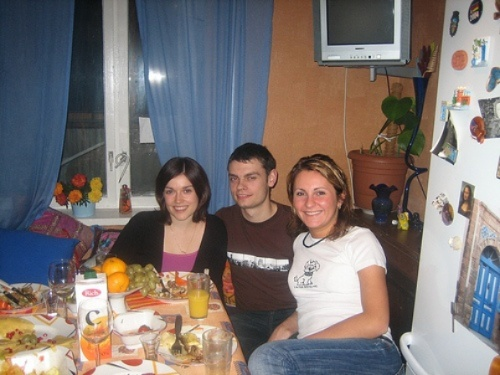
\includegraphics[width=0.24\textwidth]{figures/experiments/results_orckpt/44/0044.jpg}}
%   \hfill
%   \subfloat[Mask Prediction]{
\includegraphics[width=0.24\textwidth]{figures/experiments/results_orckpt/44/0044.png}}
%   \hfill
%   \subfloat[Grouping: Stage 1]{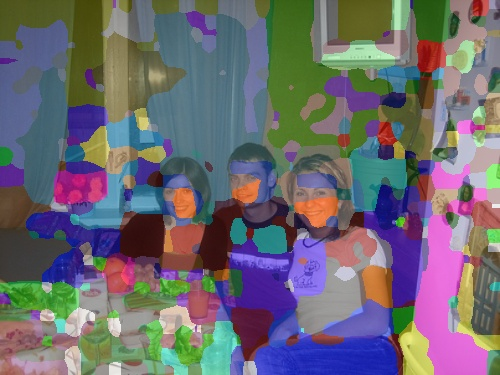
\includegraphics[width=0.24\textwidth]{figures/experiments/results_orckpt/44/0044_layer0.jpg}}
%   \hfill
%   \subfloat[Grouping: Stage 2]{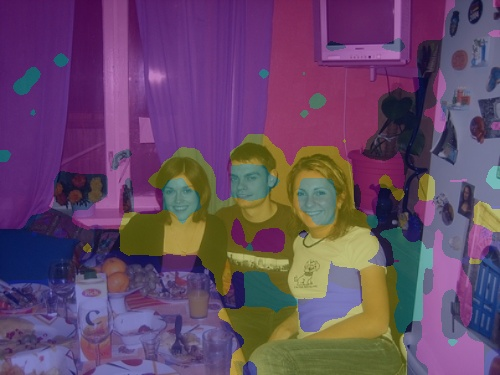
\includegraphics[width=0.24\textwidth]{figures/experiments/results_orckpt/44/0044_layer1.jpg}}
  

%   \vspace{-0.5em}
 
%   % \subfloat {\textbf{\footnotesize Image}}
%   % \hfill
%   % \subfloat {\textbf{\footnotesize \ \ \ \ \ \ \ \ \ \ \ Mask Prediction}}
%   % \hfill
%   % \subfloat {\textbf{\footnotesize Grouping: Stage 1 }}
%   % \hfill
%   % \subfloat {\textbf{\footnotesize Grouping:Stage 2}}

  
%   \vspace{-0.5em} % Add some vertical space between rows

 
%   \subfloat[Group 1]{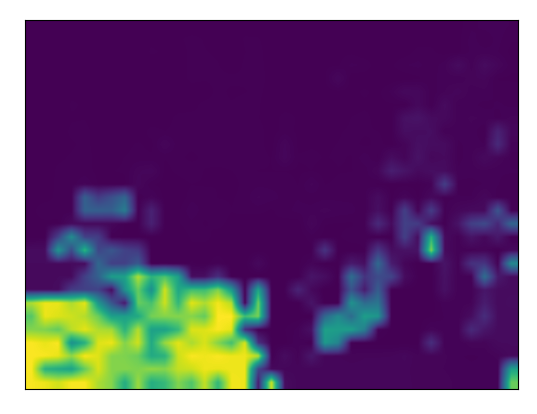
\includegraphics[width=0.24\textwidth]{figures/experiments/results_orckpt/44/attn_map0withouttitle.png}}
%   \hfill
%   \subfloat[Group 2]{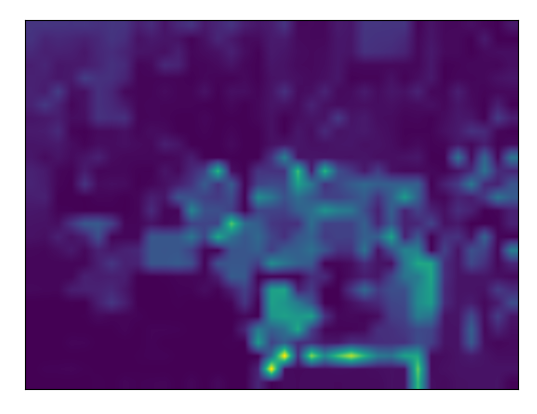
\includegraphics[width=0.24\textwidth]{figures/experiments/results_orckpt/44/attn_map1withouttitle.png}}
%   \hfill
%   \subfloat[Group 3]{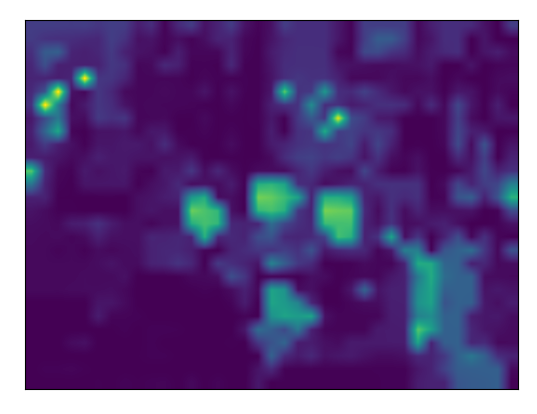
\includegraphics[width=0.24\textwidth]{figures/experiments/results_orckpt/44/attn_map2withouttitle.png}}
% \hfill
%   \subfloat[Group 4]{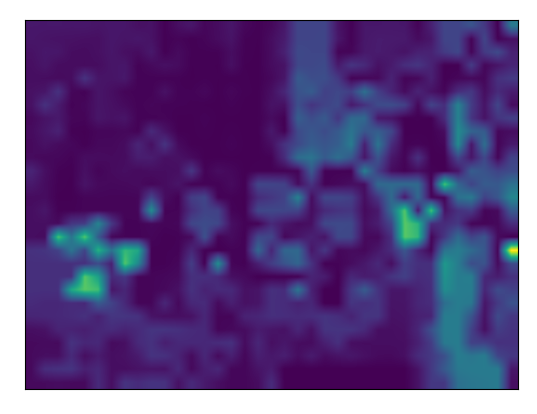
\includegraphics[width=0.24\textwidth]{figures/experiments/results_orckpt/44/attn_map3withouttitle.png}}

%    \vspace{-0.5em} % Add some vertical space between rows

 
%   \subfloat[Group 5]{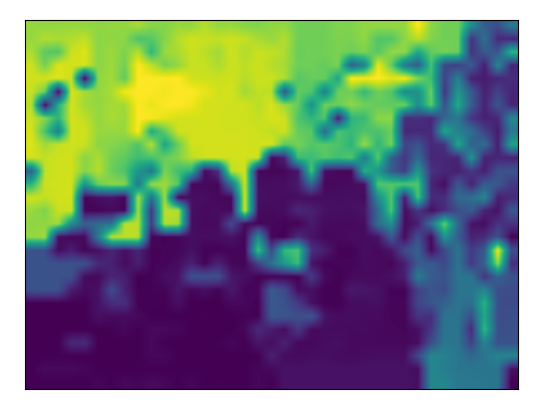
\includegraphics[width=0.24\textwidth]{figures/experiments/results_orckpt/44/attn_map4withouttitle.png}}
%   \hfill
%   \subfloat[Group 6]{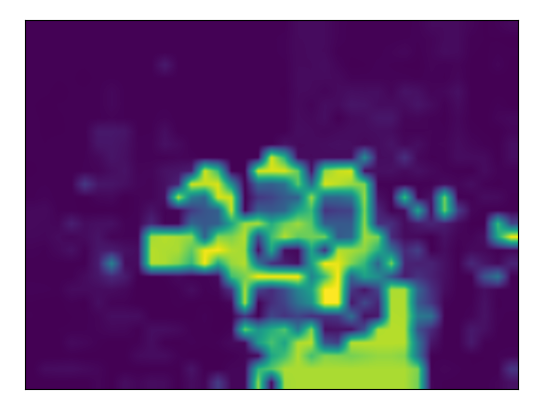
\includegraphics[width=0.24\textwidth]{figures/experiments/results_orckpt/44/attn_map5withouttitle.png}}
%   \hfill
%   \subfloat[Group 7]{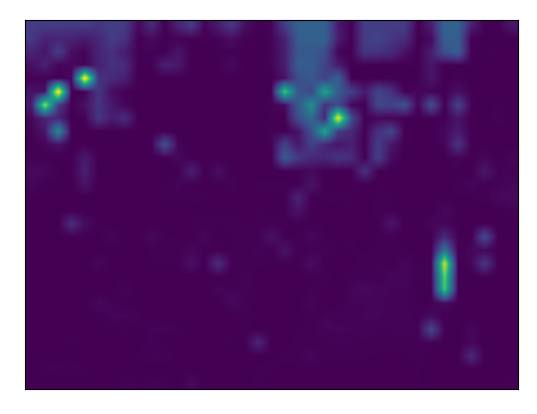
\includegraphics[width=0.24\textwidth]{figures/experiments/results_orckpt/44/attn_map6withouttitle.png}}
% \hfill
%   \subfloat[Group 8]{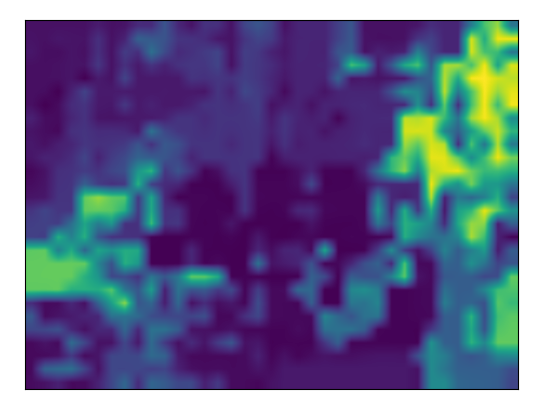
\includegraphics[width=0.24\textwidth]{figures/experiments/results_orckpt/44/attn_map7withouttitle.png}}
%   % \vspace{-0.9em}

%   \caption[\textbf{Visualization of Grouping Mechanism}]{\textbf{Visualization of Grouping Mechanism}}
%   \label{fig:group_vis}
% \end{figure}
% \documentclass{article}
% \usepackage{graphicx}
% \usepackage{subfig}

% \begin{document}

% \begin{figure}[htbp]
%   \centering
  
%   \vspace{-0.5em}
%   \subfloat[Image]{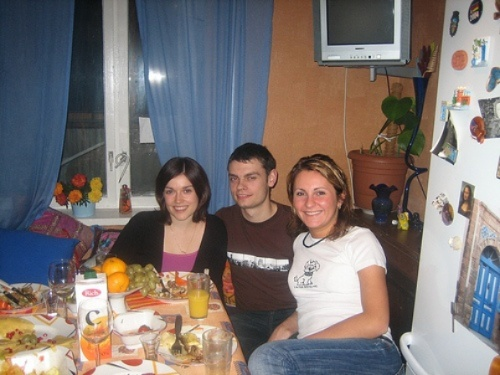
\includegraphics[width=0.24\textwidth]{figures/experiments/results_orckpt/44/0044.jpg}}
%   \hfill
%   \subfloat[Mask Prediction]{
\includegraphics[width=0.24\textwidth]{figures/experiments/results_orckpt/44/0044.png}}
%   \hfill
%   \subfloat[Grouping: Stage 1]{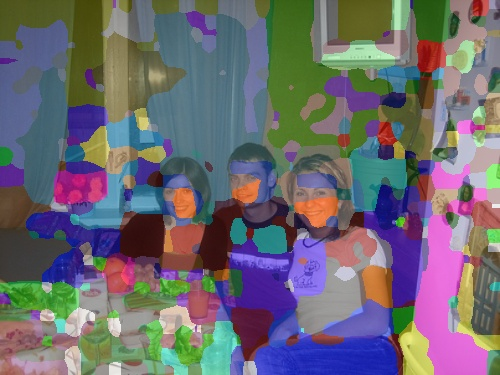
\includegraphics[width=0.24\textwidth]{figures/experiments/results_orckpt/44/0044_layer0.jpg}}
%   \hfill
%   \subfloat[Grouping: Stage 2]{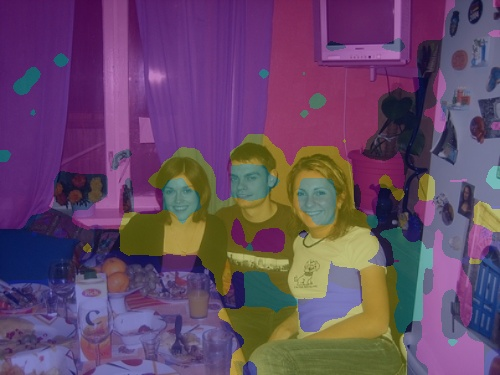
\includegraphics[width=0.24\textwidth]{figures/experiments/results_orckpt/44/0044_layer1.jpg}}
  
%   \vspace{-0.5em}
 
%   \subfloat[Group 1]{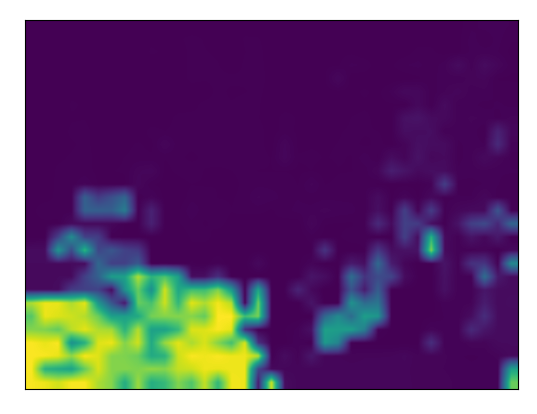
\includegraphics[width=0.24\textwidth]{figures/experiments/results_orckpt/44/attn_map0withouttitle.png}}
%   \hfill
%   \subfloat[Group 2]{\includegraphics[width=0.24\textwidth]{figures/experiments/results_orckpt/44/attn_map1withouttitle.png}}
%   \hfill
%   \subfloat[Group 3]{\includegraphics[width=0.24\textwidth]{figures/experiments/results_orckpt/44/attn_map2withouttitle.png}}
%   \hfill
%   \subfloat[Group 4]{\includegraphics[width=0.24\textwidth]{figures/experiments/results_orckpt/44/attn_map3withouttitle.png}}
  
%   \vspace{-0.5em}
 
%   \subfloat[Group 5]{\includegraphics[width=0.24\textwidth]{figures/experiments/results_orckpt/44/attn_map4withouttitle.png}}
%   \hfill
%   \subfloat[Group 6]{\includegraphics[width=0.24\textwidth]{figures/experiments/results_orckpt/44/attn_map5withouttitle.png}}
%   \hfill
%   \subfloat[Group 7]{\includegraphics[width=0.24\textwidth]{figures/experiments/results_orckpt/44/attn_map6withouttitle.png}}
%   \hfill
%   \subfloat[Group 8]{\includegraphics[width=0.24\textwidth]{figures/experiments/results_orckpt/44/attn_map7withouttitle.png}}
   
%   \vspace{-0.5em}
%   \subfloat[Image ii]{\includegraphics[width=0.24\textwidth]{figures/experiments/results_orckpt/39/0039_image.jpg}}
%   \hfill
%   \subfloat[Mask Prediction]{\includegraphics[width=0.24\textwidth]{figures/experiments/results_orckpt/39/0039.png}}
%   \hfill
%   \subfloat[Grouping: Stage 1]{\includegraphics[width=0.24\textwidth]{figures/experiments/results_orckpt/39/0039_layer0.jpg}}
%   \hfill
%   \subfloat[Grouping: Stage 2]{\includegraphics[width=0.24\textwidth]{figures/experiments/results_orckpt/39/0039_layer1.jpg}}
  
%   \vspace{-0.5em}
 
%   \subfloat[Group 1]{\includegraphics[width=0.24\textwidth]{figures/experiments/results_orckpt/39/attn_map0withouttitle.png}}
%   \hfill
%   \subfloat[Group 2]{\includegraphics[width=0.24\textwidth]{figures/experiments/results_orckpt/39/attn_map1withouttitle.png}}
%   \hfill
%   \subfloat[Group 3]{\includegraphics[width=0.24\textwidth]{figures/experiments/results_orckpt/39/attn_map2withouttitle.png}}
%   \hfill
%   \subfloat[Group 4]{\includegraphics[width=0.24\textwidth]{figures/experiments/results_orckpt/39/attn_map3withouttitle.png}}
  
%   \vspace{-0.5em}
 
%   \subfloat[Group 5]{\includegraphics[width=0.24\textwidth]{figures/experiments/results_orckpt/39/attn_map4withouttitle.png}}
%   \hfill
%   \subfloat[Group 6]{\includegraphics[width=0.24\textwidth]{figures/experiments/results_orckpt/39/attn_map5withouttitle.png}}
%   \hfill
%   \subfloat[Group 7]{\includegraphics[width=0.24\textwidth]{figures/experiments/results_orckpt/39/attn_map6withouttitle.png}}
%   \hfill
%   \subfloat[Group 8]{\includegraphics[width=0.24\textwidth]{figures/experiments/results_orckpt/39/attn_map7withouttitle.png}}

%   \caption{\textbf{Visualization of Grouping Mechanism}}
%   \label{fig:group_vis}
% \end{figure}

% \end{document}


% \begin{figure}[htbp]
%   \centering
%   \vspace{-0.5em}
 
%   \subfloat {\textbf{\footnotesize Image}}
%   \hfill
%   \subfloat {\textbf{\footnotesize \ \ \ \ \ \ \  Group 0}}
%   \hfill
%   \subfloat {\textbf{\footnotesize Image}}
%   \hfill
%   \subfloat {\textbf{\footnotesize Group 5}}

  
%   \vspace{-0.2em} % Add some vertical space between rows
  
 
%   \subfloat{\includegraphics[width=0.21\textwidth]{figures/experiments/results_orckpt/vis_groupingforclass/group0/0023.jpg}}
%   \hfill
%   \subfloat{\includegraphics[width=0.22\textwidth]{figures/experiments/results_orckpt/vis_groupingforclass/group0/23_attn_map0withouttitle.png}}
%   \hfill
%   \subfloat{\includegraphics[width=0.21\textwidth]{figures/experiments/results_orckpt/vis_groupingforclass/group5/0007.jpg}}
%   \hfill
%   \subfloat{\includegraphics[width=0.22\textwidth]{figures/experiments/results_orckpt/vis_groupingforclass/group5/0007_attn_map5withouttitle.png}}

%   \hfill
%   \subfloat{\includegraphics[width=0.22\textwidth]{figures/experiments/results_orckpt/vis_groupingforclass/group0/0034.jpg}}
%   \hfill
%   \subfloat{\includegraphics[width=0.22\textwidth]{figures/experiments/results_orckpt/vis_groupingforclass/group0/34_attn_map0withouttitle.png}}
%   \hfill
%   \subfloat{\includegraphics[width=0.22\textwidth]{figures/experiments/results_orckpt/vis_groupingforclass/group7/0031.jpg}}
%   \hfill
%   \subfloat{\includegraphics[width=0.22\textwidth]{figures/experiments/results_orckpt/vis_groupingforclass/group5/31_attn_map5withouttitle.png}}

%   \caption{\textbf{Visualization of Group Tokens}}
%   \label{fig:group_vis}
% \end{figure}


\begin{figure}[htbp]
  \centering
  \vspace{-0.5em}
 
  \subfloat {\textbf{\small Image}}
  \hspace{9em}
  \subfloat {\textbf{\small Stage 1}}
  \hspace{8em}
  \subfloat {\textbf{\small Stage 2}}

  \vspace{-0.05em} % Add some vertical space between rows
 
  \subfloat{\includegraphics[width=0.33\textwidth]{Images/0000.jpg}}
  \hfill
  \subfloat{\includegraphics[width=0.33\textwidth]{Images/stage1/0000_layer0.jpg}}
  \hfill
  \subfloat{\includegraphics[width=0.33\textwidth]{Images/stage2/0000_layer1.jpg}}
  \hfill
  \subfloat{\includegraphics[width=0.33\textwidth]{Images/0009.jpg}}
  \hfill
  \subfloat{\includegraphics[width=0.33\textwidth]{Images/stage1/0009_layer0.jpg}}
  \hfill
  \subfloat{\includegraphics[width=0.33\textwidth]{Images/stage2/0009_layer1.jpg}}
  %\hfill
  % \subfloat{\includegraphics[width=0.33\textwidth]{Images/0031.jpg}}
  % \hfill
  % \subfloat{\includegraphics[width=0.33\textwidth]{Images/stage1/0031_layer0.jpg}}
  % \hfill
  % \subfloat{\includegraphics[width=0.33\textwidth]{Images/stage2/0031_layer1.jpg}}
  \hfill

  \caption[\textbf{Visualization of Emerging Segments}]{\textbf{Visualization of Emerging Segments:}.We visualize various semantically coherent concepts that arise during Stage 1, gradually converging and forming cohesive groups as they progress into Stage 2.}
  \label{fig:group_vis}
\end{figure}


 To understand the region of attention for individual group tokens we now visualize attention maps for each of them in Fig. \ref{fig:groupattnmap}. We observe that multiple pixels of an image often have varying degrees of association to different group tokens. This association of pixels with multiple group tokens raises questions about the confidence of these relationships. For instance, in Fig. \ref{fig:groupattnmap}, `the face of the woman' is associated with Group 5 as well as Group 3, and pixels representing `bottle' are associated with Group 0 and Group 7. 
 
 \subsection{Entropy of Patches over Groups}
 \label{sec:groupentropy}
 Grounding our motivation on the understanding that, ideally, each patch should align with a single group token, ensuring a clear and unambiguous association, we next 
calculate the entropy of each patch token over all the group tokens of final stage. For this, we use $\textbf{Attn} \in \mathbb{R}^{|G^2| \times |S^1|}$, obtained in Eq. \ref{eq:globalsoftattn}. Recall, $\textbf{Attn} \in \mathbb{R}^{|G^2| \times |S^1|}$ represents distribution of segment tokens over group tokens. We visualize computing entropy for a single patch token in the Eq. \ref{eq:entropy} below. 
% Specifically, we use $\textbf{Attn}_{i,j}$ to comprehend the calculation of entropy for a single patch token over the group tokens, which corresponds to a column of the attention metric across all rows of the metric, as shown in Eq. \ref{eq:entropy}.
% \begin{equation}
% \label{eq:entropy}
% H(\textbf{G}^2, \hat{\textbf{S}}^1_j) = -\sum_{i=1}^{|G^2|} \text{$\textbf{Attn}_{i,j}$}( \hat{\textbf{G}}_i^2, \hat{\textbf{S}}^1_j) \cdot \log(\text{$\textbf{Attn}_{i,j}$}(\hat{\textbf{G}}_i^2, \hat{\textbf{S}}^1_j))
% \end{equation}
\begin{equation}
\label{eq:entropy}
H(\textbf{G}^2, \textbf{S}^1_j) = -\sum_{i=1}^{|G^2|} \text{$\textbf{Attn}_{i}$} \cdot \log(\text{$\textbf{Attn}_{i}$})
\end{equation}
In this equation, $H( \textbf{G}^2, \textbf{S}^1_j,)$ will be maximized when the probabilities produced by the softmax are $1/|G^2|$, indicating that the patch token has an equal probability of association with every group token. It is important to emphasize that our objective is to minimize this entropy. To visually represent the entropy for each pixel and comprehend the entropy of semantically coherent pixels, we interpolate $\textbf{H} \in \mathbb{R}^{|G^2| \times |S^1|}$ to acquire $\textbf{H} \in \mathbb{R}^{|G^2| \times H \times W}$. Subsequently, we compute the mean across $|G^2|$ to visualize the entropy maps, as illustrated in Figure \ref{fig:entropyacrossgroups}.


While visualizing the entropy map over group tokens for an image in Fig. \ref{fig:entropyacrossgroups}, we observe high entropy for objects like `bottle' and `face' due to their association with multiple groups. Motivated by this observation, we introduce a penalty term in the loss function, referred to as the Group Entropy Penalty or Group Entropy Loss. This penalty term is calculated as the mean entropy of all patch tokens in an image, as shown in Eq. \ref{eq:GELoss}. Subsequently we take the mean penalty for the batch and employ it in conjunction with the contrastive and multi-label contrastive loss.
\begin{equation}
\label{eq:GELoss}
\textbf{GE} = \frac{1}{|S^1|} \sum_{j=1}^{|S^1|} H(\textbf{G}^2, \textbf{S}^1_j)
\end{equation}

By minimizing this entropy, we aim to enhance the clarity and consistency of the patch token-to-group token associations, ultimately improving the performance of segmenting coherent concepts together.

\begin{figure}[t]
\centering


\begin{subfigure}{0.19\textwidth}
    \centering
    \includegraphics[width=\linewidth]{Images/0009.jpg}
    \caption{Image}
\end{subfigure}
\hfill
\begin{subfigure}{0.19\textwidth}
    \centering
    \includegraphics[width=\linewidth]{Images/all group tokens/10/attn_map2withouttitle.pdf}
    \caption{Group 3}
\end{subfigure}
\hfill
\begin{subfigure}{0.19\textwidth}
    \centering
    \includegraphics[width=\linewidth]{Images/all group tokens/10/attn_map5withouttitle.pdf}
    \caption{Group 5}
\end{subfigure}
\hfill
\begin{subfigure}{0.19\textwidth}
    \centering
    \includegraphics[width=\linewidth]{Images/all group tokens/10/attn_map0withouttitle.pdf}
    \caption{Group 0}
\end{subfigure}
\hfill
\begin{subfigure}{0.19\textwidth}
    \centering
    \includegraphics[width=\linewidth]{Images/all group tokens/10/attn_map7withouttitle.pdf}
    \caption{Group 7}
\end{subfigure}
\caption[\textbf{GroupViT: Visualization of Attention Maps of Group Tokens}]{\textbf{ Visualization of attention maps of group tokens.}}
\label{fig:groupattnmap}
\end{figure}


\begin{figure}[t]
\centering


\begin{subfigure}{0.32\textwidth}
    \centering
    \includegraphics[width=\linewidth]{Images/0009.jpg}
    \caption{Image}
\end{subfigure}
\hfill
\begin{subfigure}{0.32\textwidth}
    \centering
    \includegraphics[width=\linewidth]{Images/entropymaps/entropy_mapwithoutcb.png}
    \caption{Entropy over Groups}
    
\label{fig:entropyacrossgroups}
\end{subfigure}
\hfill
\begin{subfigure}{0.32\textwidth}
    \centering
    \includegraphics[width=\linewidth]{Images/entropymaps/class_entropywithoutcb.pdf}
    \caption{Entropy over Labels}
\label{fig:entropyacrosslabels}
\end{subfigure}

\caption[\textbf{GroupViT: Visualization of Entropy Maps}]{\textbf{  Visualization of Entropy Maps.}}
\label{fig:visentropy}
\end{figure}


\subsection{Entropy of Patches over Labels}
\label{sec:LE}


% To explore this hypothesis, we initiate an evaluation of the entropy associated with patches across various categories within the dataset. For Pascal VOC, we observe in many instances, as in Fig. \ref{fig:entropyacrosslabels},  patch associations spanning multiple labels, which underscores the inherent complexity of the segmentation task.

Next, motivated by the objective to enhance the alignment between visual and textual cues, we visualize the entropy of image pixels over labels. 
To do so, we obtain $\textbf{L}_{affinity} \in \mathbb{R}^{ H \times W \times N }$, as in Eq. \ref{eq:pred}. Following this, the entropy of all pixels over labels is calculated as demonstrated in Eq. \ref{eq:lentropy}. Here $\textbf{P}_i$ is the representation of a pixel.


\begin{equation}
\label{eq:lentropy}
H(\textbf{P}_i, \textbf{T}) = -\sum_{j=1}^{N} \textbf{$L_{affinity}$} \cdot \log(\textbf{$L_{affinity}$})
\end{equation}

The resulting visualization of this entropy distribution is presented in Fig. \ref{fig:entropyacrosslabels}. Given the observation of elevated entropy values in specific object regions, such as a woman's face, we introduce a novel loss function termed the `Label Entropy Regularization penalty', denoted as \(LE\) and defined in Eq. \ref{eq:LELoss}. This penalty aims to reduce the entropy of each patch token over the extracted labels during training.
% To do so, we calculate $\ddot{\textbf{A}}_{ST}$ as in Eq. \ref{eq:softmaxsimmat}.
During training, we obtain  $\textbf{A}_{ST} \in \mathbb{R}^{|S^3| \times N}$ in Eq. \ref{eq:simmat}, where N would be number of labels extracted. For clarity, in this context, we will use `K' to denote the number of extracted labels instead of `N' which was used in Section \ref{sec:inf} to represent the number of classes. Next we use $\text{\textbf{Attn}} \in \mathbb{R}^{|G^2| \times |S^1|}$, obtained in Eq. \ref{eq:globalsoftattn} to obtain $\textbf{T}_{affinity} \in \mathbb{R}^{|S^1| \times K}$, as shown in Eq. \ref{eq:labelentropy}. Next, we calculate entropy of each patch token over labels, as shown in Eq. \ref{eq:LELoss}. 
% of entropy of a single patch token over the text tokens, i.e. a single row of segment token $\hat{\textbf{S}}_i$  over all the columns $\textbf{T}_j$, with j ranging from 1 to K to represent K extracted texts,
% we use $\textbf{T_{affinity}}^T_{i,j}$ to understand  in Eq. \ref{eq:entropy}. 
% Recall, this operation is feasible as $|S^3|$ is equal to $|G^2|$
\begin{equation}
\label{eq:labelentropy}
\mathbf{T}_{\text{affinity}} = \text{\textbf{Attn}}^T \cdot \text{Softmax}({\textbf{A}}_{ST})
\end{equation}

\begin{align}
H(\textbf{S}^1_i, \textbf{T}) &= -\sum_{j=1}^{K} \textbf{$\textbf{T}_{affinity}$} \cdot \log(\textbf{$\textbf{T}_{affinity}$}) \\
\label{eq:LELoss}
\textbf{LE} &= \frac{1}{|S^1|} \sum_{i=1}^{|S^1|} H(\textbf{S}^1_i, \textbf{T})
\end{align}

% \begin{equation}
% \label{eq:LELoss}
% H(\textbf{S}^1_i, \textbf{T}) = -\sum_{j}^{K} \textbf{$T_{affinity}$} \cdot \log(\textbf{$T_{affinity}$})
% \end{equation}
% \begin{equation}
% \label{eq:LELoss}
% \textbf{GE} = \frac{1}{|S^1|} \sum_{j=1}^{|S^1|} H(\textbf{S}^1_i, \textbf{T})
% \end{equation}

This penalty aims to refine the alignment of information from both the modalities at earlier stages which could potentially improve performance for a task of finer granularity.
We take an average of entropy of all patch tokens of an image and subsequently take a mean of the penalty for the batch. We employ this loss in conjunction with contrastive and multi-label contrastive loss.
% \begin{equation}
% \label{eq:LELoss}
% H(\hat{\textbf{S}}^1_i, \textbf{T}_K) = -\sum_{j=1}^{|K|} \textbf{T}_{\text{affinity}}(\hat{\textbf{S}}^1_i, \textbf{T}_j) \cdot \log(\textbf{T}_{\text{affinity}}(\hat{\textbf{S}}^1_i, \textbf{T}_j))
% \end{equation}

\begin{figure}[t]
  \centering
  \includegraphics[width=1\textwidth]{Images/entropy.drawio (8).drawio (4).png}
  \caption[\textbf{Training Pipeline for Entropy Regularization}]{\textbf{Training Pipeline for Entropy Regularization}. We employ global attention to calculate entropy over Group Tokens, which is known as Group Entropy Loss (GE). We use a segment affinity metric to calculate entropy values for both Groups and Labels, collectively referred to as Entropy over Segment Affinity Metric (SE). Additionally, we calculate entropy over labels by using $T_{affinity}$, referred to as Label Entropy Loss (LE). }
  \label{fig:erfig}
\end{figure}

\subsection{Entropy over Segment Affinity Metric}
\label{sec:tier}
We introduce an entropy penalty for the `segment affinity metric' computed in the joint embedding space, drawing inspiration from the work of Palepu et al. \cite{palepu2022tier}.
% The process begins by computing the similarity between the final grouped image embedding obtained in Eq. \ref{eq:imgprojbeforeavgpool}, denoted as \(K_I \in \mathbb{R}^{{\hat{S}_i}^3 \times D_J}\), and the text embeddings obtained in Eq. \ref{eq:textproj}, denoted as \(Z_T \in \mathbb{R}^{{K} \times D_J}\), after normalizing the embeddings along the dimensional space. Here, K is the number of labels.
First we obtain the metric, denoted as $A_{ST}$, as shown in Eq. \ref{eq:simmat}.
% \begin{equation}
% \begin{aligned}
% \label{eq:simmat}
% \centering
% sim\_mat &= K_I @ Z_T
% \end{aligned}
% \end{equation}

Next, we apply a row-wise softmax to $A_{ST}$ and compute the entropy between a group token \(G_i\) and all of the label embeddings, as illustrated in Eq. \ref{eq:tierimg}.
\begin{equation}
\begin{aligned}
\label{eq:tierimg}
\text{dist}_{\text{groups}} &= \text{Softmax}(A_{ST}, \text{dim}=-1) \\
H(\textbf{G}^2_i, \textbf{T}) &= -\sum_{j}^{K} \text{dist}_{\text{groups}} \cdot \log(\text{dist}_{\text{groups}})
\end{aligned}
\end{equation}

Here, \(H(\textbf{G}^2_i, \textbf{T})\) will be maximized when the probabilities produced by the softmax are \(1/K\), indicating that the group has an equal probability of association with every label. It's important to note that our objective is to minimize this entropy.

Subsequently, we apply the same procedure to the columns of $A_{ST}$, we obtain column-wise softmax, followed by entropy calculation for each label embedding over segment embeddings, as depicted in Eq. \ref{eq:tiertxt}:
\begin{equation}
\begin{aligned}
\label{eq:tiertxt}
\text{dist}_{\text{labels}} &= \text{Softmax}(A_{ST}, \text{dim}=-2) \\
H(\textbf{G}^2, \textbf{T}^1_j) &= -\sum_{i=1}^{|G^2|}  \text{dist}_{\text{labels}} \cdot \log(\text{dist}_{\text{labels}})
\end{aligned}
\end{equation}


These obtained entropy terms are introduced as penalties in our GroupViT method to observe their impact on performance. Additionally, \(H(\textbf{G}^2_i, \textbf{T})\) is scaled by a factor of 0.2, and \(H(\textbf{G}^2, \textbf{T}^1_j)\) is scaled by a factor of 0.1 to balance their contributions to the final loss term, denoted by SE, in Eq. \ref{eq:SELoss}, following the approach by Palepu et al.
% \begin{equation}
% \label{eq:SELoss}
% \textbf{SE} = 0.2(H(\textbf{G}^2_i, \textbf{T})) + 0.1(H(\textbf{G}^2, \textbf{T}^1_j))
% \end{equation}
\begin{equation}
\label{eq:SELoss}
\textbf{SE} = 0.2(\frac{1}{|G^2|} \sum_{i=1}^{|G^2|} H(\textbf{G}_i^2, \textbf{T})
) + 0.1(\frac{1}{K} \sum_{j=1}^{K}H(\textbf{G}^2, \textbf{T}^1_j))
\end{equation}

 % \section{Visual Text Aligned Loss}
 % \label{sec:TACL}
 % The authors of PACL, Mukhoti, Jishnu, et al., demonstrated the impressive performance of CLIP in segmentation tasks through the utilization of a similarity function with the InfoNCE Contrastive Loss \cite{oord2018representation}.This approach aligned image patches with text, achieving finer granularity \cite{mukhoti2023open}. 
 % % However, GroupViT's alignment mechanism, which aligns patch tokens with grouping tokens to encourage the emergence of semantically coherent concepts, does not consider the alignment of text tokens or their similarity with grouping tokens until the final stage. We again propose that exploring the integration of modalities across different stages for finer-grained tasks.
 % Motivated by this, and while constrained by architectural parameters such as differing dimensions for visual and text encoders (384 and 256 dimensions respectively), we investigate alignment after projection within a common latent space. To achieve this, in addition to employing the average pooling technique described in Equation \ref{eq:avgpool}, we also project the grouping tokens to the latent space using the same image projector, as shown in Equation \ref{eq:imgprojbeforeavgpool}. This produces a set of ${\textbf{K}^I} \in \mathbb{R}^{|S^3| \times D_J}$, with $|S^3|$ representing the number of segments after the third and final stage.
 % $ embeddings, where $g$ ranges from 1 to 8, signifying the number of segmented tokens attained after the final stage of the visual encoder, as presented in Equation \ref{eq:groupproj}.
 % However to retain the knowledge of pre-trained model and restrained by architectural constraints, for instance different width of visual and text encoders with 384 and 256 dimensionality respectively, we continue to explore alignment after projection in the common latent space. To do so, besides taking the average pool as described in the equation \ref{eq:avgpool}, we also project the grouping tokens to the latent space using the same image projector as shown in Equation:\ref{eq:imgproj}. Therefore we obtain $Z_g$, where $g \in {1,...,8}$ where 8 is the number of segmentaed tokens we obtain after the last stage of visual encoder as shown in the below Eq:\ref{eq:groupproj}
%  \begin{equation}
% \label{eq:groupproj}
%     \{Z_g\} = \text{MLP}( \{S_i^{3}\})
% \end{equation}
% Subsequently, we compute the cosine similarity between $\textbf{K}^I$ and $\textbf{Z}^T$, obtained from Equations \ref{eq:imgprojbeforeavgpool} and \ref{eq:textproj} respectively, as illustrated in Equation \ref{eq:cosinesim}.
%  \begin{equation}
% \label{eq:cosinesim}
%     S(I,T) = \textbf{K}^I \cdot \text{Transpose}(\textbf{Z}^T)
% \end{equation}
% The resulting probability distribution from this similarity calculation is then utilized to weigh the group token embeddings, leading to the formulation presented in Equation \ref{eq:weightedgroupembed}.
%  \begin{equation}
% \label{eq:weightedgroupembed}
%     \textbf{W}^{I} = \textbf{Z}^I.(\text{Softmax}(S(I, T)))
% \end{equation}
% These weighted final embeddings, rather than average-pooled embeddings, are subsequently employed to calculate both the contrastive loss and the multi-label contrastive loss, as explained in Equations \ref{eq:cl} and \ref{eq:mll} respectively.

% \section{OV Segmentator}
% One of the drawbacks for GroupViT is visual variance. A model introduced  by Xu, Jilan, et al, called OVSegmentator claimed to solve the problem of visual variance by  adding proxy tasks for the image-text training. Similar to GroupViT, they train image-text pair in a transformer-based architecture. Akin to GroupViT, they also introduced a binding module to assemble the semantically coherent image pixels into a set of learnable group tokens via a binding module, then aligns the group tokens to corresponding caption embeddings. There are a few modification on the top of global-image-text pair to solve issues such as visual variance.
% First, they use two proxy tasks in conjunction with the regular global image-text pair training with contrastive loss. (i) masked entity completion: The former
% trains the model to infer all the masked entities in the sentence given the group tokens, and (ii) cross-image mask consistency, enforces consistent mask prediction for images with the common entity. Second,They filter CC12M dataset keeping the entities having high frequency, to CC4M dataset to train the model for open-vocabulary segmentation which they claim to improve the training efficiency. 
% They claim that introducing these two modification has made the model more robust for learning entity-specific, fine-grained and visually invariant groups.
% Similar to GroupViT, OVSegmentator has a transformer based vision-encoder and text-encoder. The visual encoder consists of two components, namely,
% Transformer encoders and a slot-attention \cite{locatello2020object} based binding module. This binding module is similar to the grouping block used in GroupViT \ref{sec:gvitarch}. It is different that cross-attention in transformer as it normalizes query before performing cross-attention. The binding module is placed between 
%  a stack of 6 transformer block. The author initialized the transformer block of Vision encoder by DINO\cite{caron2021emerging} weights pre-trained on ImageNet\cite{deng2009imagenet}. For Text encoder, they use 12 trasnformer block initialized with pre-trained model of BERT \cite{devlin2018bert} as a text encoder pretrained on pre-trained on BookCorpus\cite{zhu2015aligning} and English Wikipedia. 
% Specifically the image tokens and learnable group tokens are concatenated, and iterative processed by the Transformer encoders, and a binding module with slot-attention isadopted for grouping .Moreover for caption, authors use raw caption, denoted as ${\mathcal{T}_{R}}$, masked caption, denotes as ${\mathcal{T}_{M}}$,  where they mask specific entities and Prompted entity, denotes as ${\mathcal{T}_{E}}$, where they prompt the masked emitty with a simple template: 'A photo of a $\{Entity_1\}$ and $\{Entity_2\}$ and $...\{Entity_n\}$'. Ovsegmentator trains image-text pair with contrastive loss as in GroupViT. Additionally, it employs two additional loss function for the proxy tasks.

% \subsection{Masked Entity Compeltion}
% OVSegmentator maintains a bank of 100 frequently appearing entities using NLTK toolkit, denotes as \(\Omega = \Phi_{entity}(\{T_1, \ldots, T_N\})\), where $T_1, \ldots T_N$ represents entities such as 'person', 'car', etc. This is done so that abstract nouns such as 'art', 'view', etc. can't be part of the masked text as they don't represent any semantic concept in an image. As seen in the Figure \ref{ovseg}, we use a masked entity loss function called 

% The goal of masked entity completion is to infer all the masked entities in the sentence given the group tokens. In specific, authors use a transformer based decoder module  to perform cross-attention between projection of masked caption embedding as query and  two linear transformations
% of group tokens are treated as key and values, respectively.

% \begin{equation}
%    \hat{{\mathcal{T}_{M}}} = \text{Binding\_Module}(W_{Q} \mathcal{T}_{M}, W_{K} G, W_{V} \cdot G)
% \end{equation}
% % \begin{equation}
% %     \mathcal{T}_{m-cap} = (\text{Slot-Attention}, (W_V \cdot G) \cdot T) 
    
% % \end{equation}
% The obtained masked-caption embedding is then passed through one block of self-attention block. Lastly, we extract the [EOT] token features, denoted as $z_{M}$ and $z_{E}$ from $\hat{{\mathcal{T}_{M}}}$ and ${\mathcal{T}_{E}}$, and construct a contrastive loss as shown in below Eq. \ref{eq:entityloss}

% \begin{equation}
% \label{eq:entityloss}
% L_{\text{entity}} = \frac{1}{2} \left( \exp(z_{M_i} \cdot z_{E_i}) \frac{1}{P_l} \exp(z_{M_i} \cdot z_{E_l}) + \exp(z_{M_i} \cdot z_{E_i}) \frac{1}{P_l} \exp(z_{M_l} \cdot z_{E_i}) \right)
% \end{equation}

% \subsection{Cross-image Mask Consistency.}
% \todo{Ask Maria , do we really have to write about ti as we are not using it for finetuning? and how much}

% \begin{figure*}[tbh!]
% \label{ovseg}
%   \centering
%   \includegraphics[width=1\textwidth]{Images/model.png}
%   \caption{\textbf{Figure is adapted from OVsegmentator\cite{xu2023learning}}. Architecture of OVSegmentator:The model takes an image-text pair as input, and outputs the image features and a set of learnable group
% tokens, which is aligned to the caption embedding via Lcontrast. The visual encoder consists of Transformer encoder layers, with a slotattention based binding module in between to cluster the image tokens into groups. To enrich group semantics, (1) Lentity trains the model to infer all masked entities in the caption given the group tokens. (2) Lmask enforces consistent mask predictions of images with the same
% entity (right figure). During inference, only visual and text encoders and learned group tokens are used to generate the segmentation mask}
%   \label{fig:ovseg}
% \end{figure*}


